\documentclass[10pt,a4paper]{article}
\usepackage[UTF8,fontset = windows]{ctex}
\setCJKmainfont[BoldFont=黑体,ItalicFont=楷体]{华文中宋}
\usepackage{amssymb,amsmath,amsfonts,amsthm,mathrsfs,dsfont,graphicx}
\usepackage{ifthen,indentfirst,enumerate,color,titletoc}
\usepackage{tikz}
\usepackage{multicol}
\usepackage{makecell}
\usepackage{longtable}
\usetikzlibrary{arrows,calc,intersections,patterns,decorations.pathreplacing,3d,angles,quotes,positioning}
\usepackage[bf,small,indentafter,pagestyles]{titlesec}
\usepackage[top=1in, bottom=1in,left=0.8in,right=0.8in]{geometry}
\renewcommand{\baselinestretch}{1.65}
\newtheorem{defi}{定义~}
\newtheorem{eg}{例~}
\newtheorem{ex}{~}
\newtheorem{rem}{注~}
\newtheorem{thm}{定理~}
\newtheorem{coro}{推论~}
\newtheorem{axiom}{公理~}
\newtheorem{prop}{性质~}
\newcommand{\blank}[1]{\underline{\hbox to #1pt{}}}
\newcommand{\bracket}[1]{(\hbox to #1pt{})}
\newcommand{\onech}[4]{\par\begin{tabular}{p{.9\textwidth}}
A.~#1\\
B.~#2\\
C.~#3\\
D.~#4
\end{tabular}}
\newcommand{\twoch}[4]{\par\begin{tabular}{p{.46\textwidth}p{.46\textwidth}}
A.~#1& B.~#2\\
C.~#3& D.~#4
\end{tabular}}
\newcommand{\vartwoch}[4]{\par\begin{tabular}{p{.46\textwidth}p{.46\textwidth}}
(1)~#1& (2)~#2\\
(3)~#3& (4)~#4
\end{tabular}}
\newcommand{\fourch}[4]{\par\begin{tabular}{p{.23\textwidth}p{.23\textwidth}p{.23\textwidth}p{.23\textwidth}}
A.~#1 &B.~#2& C.~#3& D.~#4
\end{tabular}}
\newcommand{\varfourch}[4]{\par\begin{tabular}{p{.23\textwidth}p{.23\textwidth}p{.23\textwidth}p{.23\textwidth}}
(1)~#1 &(2)~#2& (3)~#3& (4)~#4
\end{tabular}}
\begin{document}

\begin{enumerate}[1.]

\item { (000001)}用列举法表示下列集合:\\
(1) 十二生肖组成的集合;\\
(2) 中国国旗上所有颜色组成的集合.


关联目标:

K0102001B|D01001B|能在具体情境中用列举法描述集合.



标签: 第一单元

答案: 暂无答案

解答或提示: 暂无解答与提示

使用记录:

暂无使用记录


出处: 教材复习题
\item { (000002)}用描述法表示下列集合:\\
(1) 平面直角坐标系中第一象限的角平分线上的所有点组成的集合;\\
(2) $3$的所有倍数组成的集合.


关联目标:

K0102002B|D01001B|能在具体情境中用描述法描述集合.



标签: 第一单元

答案: 暂无答案

解答或提示: 暂无解答与提示

使用记录:

暂无使用记录


出处: 教材复习题
\item { (000004)}已知方程$x^2+px+4=0$的所有解组成的集合为$A$, 方程$x^2+x+q=0$的所有解组成的集合为$B$, 且$A\cap B=\{4\}$. 求集合$A\cup B$的所有子集.


关联目标:

K0104001B|D01001B|理解两个集合的交集的含义, 在具体数学情境中, 能求两个集合的交集.

K0104003B|D01001B|理解两个集合的并集的含义, 在具体数学情境中, 能求两个集合的并集.

K0103001B|D01001B|理解集合之间包含的概念, 能识别给定集合的子集.



标签: 第一单元

答案: 暂无答案

解答或提示: 暂无解答与提示

使用记录:

暂无使用记录


出处: 教材复习题
\item { (000005)}已知集合$A=(-2, 1)$, $B=(-\infty, -2)\cup [1, +\infty)$. 求: $A\cup B$, $A\cap B$.


关联目标:

K0102004B|D01001B|会用区间表示一些实数集合.

K0104001B|D01001B|理解两个集合的交集的含义, 在具体数学情境中, 能求两个集合的交集.

K0104003B|D01001B|理解两个集合的并集的含义, 在具体数学情境中, 能求两个集合的并集.



标签: 第一单元

答案: 暂无答案

解答或提示: 暂无解答与提示

使用记录:

暂无使用记录


出处: 教材复习题
\item { (000006)}已知全集$U=(-\infty, 1)\cup [2, +\infty)$, 集合$A=(-1, 1)\cup [3, +\infty)$. 求$\overline{A}$.


关联目标:

K0104006B|D01001B|理解在给定集合中一个子集的补集的含义, 在具体数学情境中, 能求给定集合中一个子集的补集.



标签: 第一单元

答案: 暂无答案

解答或提示: 暂无解答与提示

使用记录:

暂无使用记录


出处: 教材复习题
\item { (000007)}已知集合$A=\{x|x^2+px+q=0\}$, $B=\{x|x^2-x+r=0\}$, 且$A\cap B=\{-1\}$, $A\cup B=\{-1, 2\}$. 求实数$p$、$q$、$r$的值.


关联目标:

K0104002B|D01001B|能用文氏图反映两个集合的交集.

K0104004B|D01001B|能用文氏图反映两个集合的并集.



标签: 第一单元

答案: 暂无答案

解答或提示: 暂无解答与提示

使用记录:

暂无使用记录


出处: 教材复习题
\item { (000009)}已知陈述句$\alpha$是$\beta$的充分非必要条件. 若集合$M=\{x|x\text{满足}\alpha\}$, $N=\{x|x\text{满足}\beta\}$, 则$M$与$N$的关系为\bracket{20}.
\fourch{$M\subset N$}{$M\supset N$}{$M=N$}{$M\cap N=\varnothing$}


关联目标:

K0105001B|D01002B|结合集合之间的包含关系, 理解推出关系的含义以及推出关系的传递性.

K0106001B|D01002B|知道充分条件、必要条件的定义, 充要条件的含义.



标签: 第一单元

答案: 暂无答案

解答或提示: 暂无解答与提示

使用记录:

暂无使用记录


出处: 教材复习题
\item { (000011)}若集合$M=\{a|a=x+\sqrt2y, x,y\in \mathbf{Q}\}$, 则下列结论正确的是\bracket{20}.
\fourch{$M\subseteq \mathbf{Q}$}{$M=\mathbf{Q}$}{$M\supset \mathbf{Q}$}{$M\subset \mathbf{Q}$}


关联目标:

K0103001B|D01001B|理解集合之间包含的概念, 能识别给定集合的子集.



标签: 第一单元

答案: 暂无答案

解答或提示: 暂无解答与提示

使用记录:

暂无使用记录


出处: 教材复习题
\item { (000012)}若$\alpha$是$\beta$的必要非充分条件, $\beta$是$\gamma$的充要条件, $\gamma$是$\delta$的必要非充分条件, 则$\delta$是$\alpha$的\blank{50}条件, $\gamma$是$\alpha$的\blank{50}条件.


关联目标:

K0103001B|D01001B|理解集合之间包含的概念, 能识别给定集合的子集.

K0106001B|D01002B|知道充分条件、必要条件的定义, 充要条件的含义.



标签: 第一单元

答案: 暂无答案

解答或提示: 暂无解答与提示

使用记录:

暂无使用记录


出处: 教材复习题
\item { (000013)}已知全集$U=\{x|x\text{为不大于}20\text{的素数}\}$. 若$A\cap \overline{B}=\{3, 5\}$, $\overline{A}\cap B=\{7, 19\}$, $\overline{A\cup B}=\{2, 17\}$, 则$A=$\blank{50}, $B=$\blank{50}.


关联目标:

K0104002B|D01001B|能用文氏图反映两个集合的交集.

K0104004B|D01001B|能用文氏图反映两个集合的并集.



标签: 第一单元

答案: 暂无答案

解答或提示: 暂无解答与提示

使用记录:

暂无使用记录


出处: 教材复习题
\item { (000014)}已知集合$P=\{x|-2\le x\le 5\}$, $Q=\{x|x\ge k+1\text{且}x\le 2k-1\}$, 且$Q\subseteq P$. 求实数$k$的取值范围.


关联目标:

K0103001B|D01001B|理解集合之间包含的概念, 能识别给定集合的子集.



标签: 第一单元

答案: 暂无答案

解答或提示: 暂无解答与提示

使用记录:

暂无使用记录


出处: 教材复习题
\item { (000015)}已知全集$U=\mathbf{R}$, 集合$A=\{x|x\le a-1\}$, $B=\{x|x>a+2\}$, $C=\{x|x<0\text{或}x\ge 4\}$, 且$\overline{A\cup B}\subseteq C$. 求实数$a$的取值范围.


关联目标:

K0102003B|D01001B|会选择合适的表示集合的方式, 会正确地进行表示方式的切换.

K0103001B|D01001B|理解集合之间包含的概念, 能识别给定集合的子集.



标签: 第一单元

答案: 暂无答案

解答或提示: 暂无解答与提示

使用记录:

暂无使用记录


出处: 教材复习题
\item { (000016)}已知集合$A=\{x|(a-1)x^2+3x-2=0\}$. 是否存在这样的实数$a$, 使得集合$A$有且仅有两个子集? 若存在, 求出实数$a$的值及对应的两个子集; 若不存在, 说明理由.


关联目标:

K0103001B|D01001B|理解集合之间包含的概念, 能识别给定集合的子集.

K0109001B|D01004B|会用集合表示一元二次方程的解集.



标签: 第一单元

答案: 暂无答案

解答或提示: 暂无解答与提示

使用记录:

暂无使用记录


出处: 教材复习题
\item { (000019)}已知非空数集$S$满足: 对任意给定的$x,y\in S$($x,y$可以相同), 有$x+y\in S$且$x-y\in S$.\\
(1) 哪个数一定是$S$中的元素? 说明理由;\\
(2) 若$S$是有限集, 求$S$;\\
(3) 若$S$中最小的正数为$5$, 求$S$.


关联目标:

K0105002B|D01002B|理解命题的定义, 能在熟悉的情境中运用推出关系判断条件命题的真假.

K0101002B|D01001B|理解有限集、无限集、空集的含义.

K0107003B|D01002B|了解反证法的思想以及表达方式, 能正确使用反证法证明一些简单的数学命题.



标签: 第一单元

答案: 暂无答案

解答或提示: 暂无解答与提示

使用记录:

暂无使用记录


出处: 教材复习题
\item { (000026)}求不等式$5\le x^2-2x+2<26$的所有正整数解.


关联目标:

K0114001B|D01004B|掌握结合一元二次函数的图像求解一元二次不等式的方法.

K0104001B|D01001B|理解两个集合的交集的含义, 在具体数学情境中, 能求两个集合的交集.



标签: 第一单元

答案: 暂无答案

解答或提示: 暂无解答与提示

使用记录:

暂无使用记录


出处: 教材复习题
\item { (000028)}设关于$x$的不等式$a_1x^2+b_1x+c_1>0$与$a_2x^2+b_2x+c_2>0$的解集分别为$A$、$B$,
试用集合运算表示下列不等式组的解集:\\
(1) $\begin{cases} a_1x^2+b_1x+c_1>0, \\ a_2x^2+b_2x+c_2>0;\end{cases}$\\
(2) $\begin{cases} a_1x^2+b_1x+c_1\le 0, \\ a_2x^2+b_2x+c_2>0;\end{cases}$\\
(3) $\begin{cases} a_1x^2+b_1x+c_1\le 0, \\ a_2x^2+b_2x+c_2\le 0.\end{cases}$


关联目标:

K0104001B|D01001B|理解两个集合的交集的含义, 在具体数学情境中, 能求两个集合的交集.

K0104006B|D01001B|理解在给定集合中一个子集的补集的含义, 在具体数学情境中, 能求给定集合中一个子集的补集.



标签: 第一单元

答案: 暂无答案

解答或提示: 暂无解答与提示

使用记录:

暂无使用记录


出处: 教材复习题
\item { (000037)}已知集合$A=\{x||x-a|<2\}$, $B=\{x|\dfrac{2x-1}{x+2}<1\}$, 且$A\subseteq B$. 求实数$a$的取值范围.


关联目标:

K0116002B|D01004B|会用转化为整式不等式(组)解一些简单的分式不等式.

K0117001B|D01004B|会用绝对值的几何意义求解一些基本的含绝对值的不等式.

K0103001B|D01001B|理解集合之间包含的概念, 能识别给定集合的子集.



标签: 第一单元

答案: 暂无答案

解答或提示: 暂无解答与提示

使用记录:

暂无使用记录


出处: 教材复习题
\item { (000045)}已知集合$A=\{x|x^2-2x-3>0\}$, $B=\{x|x^2+px+q\le 0\}$. 若$A\cup B=\mathbf{R}$, 且$A\cap B=[-2,-1)$, 求实数$p$及$q$的值.


关联目标:

K0104001B|D01001B|理解两个集合的交集的含义, 在具体数学情境中, 能求两个集合的交集.

K0104003B|D01001B|理解两个集合的并集的含义, 在具体数学情境中, 能求两个集合的并集.

K0115002B|D01004B|在已知解集的情形下, 会求解含参一元二次不等式系数所满足的关系或者系数值.



标签: 第一单元

答案: 暂无答案

解答或提示: 暂无解答与提示

使用记录:

暂无使用记录


出处: 教材复习题
\item { (000346)}设集合$A=\{x||x-2|<1,x\in \mathbf{R}\}$, 集合$B=\mathbf{Z}$, 则$A\cap B=$\blank{50}.


关联目标:

暂未关联目标



标签: 第一单元

答案: $\{2\}$

解答或提示: 暂无解答与提示

使用记录:

20211203	2022届高三1班	\fcolorbox[rgb]{0,0,0}{1.000,0.140,0}{0.930}


出处: 赋能练习
\item { (000356)}若集合$A=\{x|y^2=x,y\in \mathbf{R}\}$, $B=\{y|y=\sin x,x\in \mathbf{R}\}$, 则$A\cap B=$\blank{50}.


关联目标:

暂未关联目标



标签: 第一单元

答案: $[0,1]$

解答或提示: 暂无解答与提示

使用记录:

20211210	2022届高三1班	\fcolorbox[rgb]{0,0,0}{1.000,0.182,0}{0.909}


出处: 赋能练习
\item { (000377)}设全集$U=\mathbf{R}$, 集合$A=\{-1,0,1,2,3\}$, $B=\{x|x\ge 2\}$, 则$A\cap {\complement_U}B=$\blank{50}.


关联目标:

暂未关联目标



标签: 第一单元

答案: $\{-1,0,1\}$

解答或提示: 暂无解答与提示

使用记录:

20211223	2022届高三1班	\fcolorbox[rgb]{0,0,0}{1.000,0.000,0}{1.000}


出处: 赋能练习
\item { (000386)}设集合$M=\{x|x^2=x\}$, $N=\{x|\lg x\le 0\}$, 则$M\cap N=$\blank{50}.


关联目标:

暂未关联目标



标签: 第一单元

答案: $\{1\}$

解答或提示: 暂无解答与提示

使用记录:

20211230	2022届高三1班	\fcolorbox[rgb]{0,0,0}{1.000,0.090,0}{0.955}


出处: 赋能练习
\item { (000397)}已知集合$A=\{x|\dfrac12\le {2^x}<16\}$, $B=\{x|y=\log _2(9-x^2)\}$, 则$A\cap B=$\blank{50}.


关联目标:

暂未关联目标



标签: 第一单元

答案: $[-1,3)$

解答或提示: 暂无解答与提示

使用记录:

20211231	2022届高三1班	\fcolorbox[rgb]{0,0,0}{1.000,0.136,0}{0.932}


出处: 赋能练习
\item { (000416)}已知$U=\mathbf{R}$, 集合$A=\{x|4-2x\ge x+1\}$, 则${\complement_U}A=$\blank{50}.


关联目标:

暂未关联目标



标签: 第一单元

答案: $\{x|x>1\}$

解答或提示: 暂无解答与提示

使用记录:

20220106	2022届高三1班	\fcolorbox[rgb]{0,0,0}{1.000,0.000,0}{1.000}


出处: 赋能练习
\item { (000426)}已知集合$A=\{1,2,4,6,8\}$, $B=\{x|x=2k,k\in A\}$, 则$A\cap B=$\blank{50}.


关联目标:

暂未关联目标



标签: 第一单元

答案: $\{2,4,8\}$

解答或提示: 暂无解答与提示

使用记录:

20220111	2022届高三1班	\fcolorbox[rgb]{0,0,0}{1.000,0.046,0}{0.977}


出处: 赋能练习
\item { (000446)}若集合$M=\{x|{x^2}-2x<0\}$, $N=\{x||x|>1\}$, 则$M\cap N=$\blank{50}.


关联目标:

暂未关联目标



标签: 第一单元

答案: $(1,2)$

解答或提示: 暂无解答与提示

使用记录:

20220221	2022届高三1班	\fcolorbox[rgb]{0,0,0}{1.000,0.000,0}{1.000}


出处: 赋能练习
\item { (000456)}设集合$A=\{2,3,4,12\}$, $B=\{0,1,2,3\}$, 则$A\cap B=$\blank{50}.


关联目标:

暂未关联目标



标签: 第一单元

答案: $\{2,3\}$

解答或提示: 暂无解答与提示

使用记录:

20220222	2022届高三1班	\fcolorbox[rgb]{0,0,0}{1.000,0.000,0}{1.000}


出处: 赋能练习
\item { (000466)}已知集合$A=\{1,2,5\}$, $B=\{2,a\}$. 若$A\cup B=\{1,2,3,5\}$, 则$a=$\blank{50}.


关联目标:

暂未关联目标



标签: 第一单元

答案: $3$

解答或提示: 暂无解答与提示

使用记录:

20220223	2022届高三1班	\fcolorbox[rgb]{0,0,0}{1.000,0.000,0}{1.000}


出处: 赋能练习
\item { (000476)}已知全集$U=\mathbf{N}$, 集合$A=\{1,2,3,4\}$, 集合$B=\{3,4,5\}$, 则$(\complement_U A)\cap B=$\blank{50}.


关联目标:

暂未关联目标



标签: 第一单元

答案: $\{5\}$

解答或提示: 暂无解答与提示

使用记录:

20220224	2022届高三1班	\fcolorbox[rgb]{0,0,0}{1.000,0.046,0}{0.977}


出处: 赋能练习
\item { (000496)}已知全集$U=\mathbf{R}$, 集合$A=\{x||x-1|>1\}$, $B=\{x|\dfrac{x-3}{x+1}<0\}$, 则$(\complement_U A)\cap B=$\blank{50}.


关联目标:

暂未关联目标



标签: 第一单元

答案: $[0,2]$

解答或提示: 暂无解答与提示

使用记录:

20220228	2022届高三1班	\fcolorbox[rgb]{0,0,0}{1.000,0.142,0}{0.929}


出处: 赋能练习
\item { (000506)}若全集$U=\mathbf{R}$, 集合$A=\{x|x\le 0\text{或} x\ge 2\}$, 则$\complement_U A=$\blank{50}.


关联目标:

暂未关联目标



标签: 第一单元

答案: $A=\{x|0<x<2\}$

解答或提示: 暂无解答与提示

使用记录:

20220302	2022届高三1班	\fcolorbox[rgb]{0,0,0}{1.000,0.000,0}{1.000}


出处: 赋能练习
\item { (000526)}集合$P=\{x|0 \le x<3, x\in \mathbf{Z}\}$, $M=\{x|x^2 \le 9\}$, 则$P\cap M=$\blank{50}.


关联目标:

暂未关联目标



标签: 第一单元

答案: $\{ 0,1,2 \}$

解答或提示: 暂无解答与提示

使用记录:

20220304	2022届高三1班	\fcolorbox[rgb]{0,0,0}{1.000,0.364,0}{0.818}


出处: 赋能练习
\item { (000536)}设全集$U=\{ 1,2,3,4,5\}$, 若集合$A=\{3,4,5\}$, 则$\complement_U A=$\blank{50}.


关联目标:

暂未关联目标



标签: 第一单元

答案: $\{1,2\}$

解答或提示: 暂无解答与提示

使用记录:

20220307	2022届高三1班	\fcolorbox[rgb]{0,0,0}{1.000,0.000,0}{1.000}


出处: 赋能练习
\item { (000547)}已知集合$A=\{x|0<x<3\}$, $B=\{x|x^2\ge 4\}$, 则$A\cap B=$\blank{50}.


关联目标:

暂未关联目标



标签: 第一单元

答案: $[2,3)$

解答或提示: 暂无解答与提示

使用记录:

20220309	2022届高三1班	\fcolorbox[rgb]{0,0,0}{1.000,0.046,0}{0.977}


出处: 赋能练习
\item { (000556)}设全集$U=\mathbf{Z}$, 集合$M=\{1,2\}$, $P=\{-2,-1,0,1,2\}$, 则$P\cap \complement_U M$=\blank{50}.


关联目标:

暂未关联目标



标签: 第一单元

答案: $\{-2,-1,0\}$

解答或提示: 暂无解答与提示

使用记录:

20220310	2022届高三1班	\fcolorbox[rgb]{0,0,0}{1.000,0.000,0}{1.000}


出处: 赋能练习
\item { (000576)}已知集合$A=\{1,2,m\}$, $B=\{3,4\}$.若$A\cap B=\{3\}$, 则实数$m=$\blank{50}.


关联目标:

暂未关联目标



标签: 第一单元

答案: $-\frac 35$

解答或提示: 暂无解答与提示

使用记录:

20220316	2022届高三1班	\fcolorbox[rgb]{0,0,0}{1.000,0.046,0}{0.977}


出处: 赋能练习
\item { (000596)}设全集$U=\{1,2,3,4\}$, 集合$A=\{x|x^2-5x+4<0,x\in \mathbf{Z}\}$, 则$\complement_U A$=\blank{50}.


关联目标:

暂未关联目标



标签: 第一单元

答案: $\{1,4\}$

解答或提示: 暂无解答与提示

使用记录:

20220323	2022届高三1班	\fcolorbox[rgb]{0,0,0}{1.000,0.140,0}{0.930}


出处: 赋能练习
\item { (000617)}已知集合$M=\{x||x+1|\le 1\},N=\{-1,0,1\},$则$M\cap N=$\blank{50}.


关联目标:

暂未关联目标



标签: 第一单元

答案: $\{-1,0\}$

解答或提示: 暂无解答与提示

使用记录:

20220325	2022届高三1班	\fcolorbox[rgb]{0,0,0}{1.000,0.046,0}{0.977}


出处: 赋能练习
\item { (000627)}若全集$U=\mathbf{R}$, 集合$A=\{x|x\ge 1\}\cup\{x|x<0\}$, 则$\complement_U A=$\blank{50}.


关联目标:

暂未关联目标



标签: 第一单元

答案: $[0,1)$

解答或提示: 暂无解答与提示

使用记录:

20220329	2022届高三1班	\fcolorbox[rgb]{0,0,0}{1.000,0.000,0}{1.000}


出处: 赋能练习
\item { (000636)}集合$A=\{1,2,3,4\}$, $B=\{x|(x-1)(x-5)<0\}$, 则$A\cap B=$\blank{50}.


关联目标:

暂未关联目标



标签: 第一单元

答案: $\{2,3,4\}$

解答或提示: 暂无解答与提示

使用记录:

20220330	2022届高三1班	\fcolorbox[rgb]{0,0,0}{1.000,0.000,0}{1.000}


出处: 赋能练习
\item { (000666)}已知集合$A=\{x|\dfrac{x-2}{x+1}\ge 0\}$, 集合$B=\{y|0 \le y<4\}$, 则$A\cap B$=\blank{50}.


关联目标:

暂未关联目标



标签: 第一单元

答案: $[2,4)$

解答或提示: 暂无解答与提示

使用记录:

20220408	2022届高三1班	\fcolorbox[rgb]{0,0,0}{1.000,0.094,0}{0.953}


出处: 赋能练习
\item { (000686)}已知集合$A=\{x|x>-1, \ x\in \mathbf{R}\}$, 集合$B=\{x|x<2, \ x\in \mathbf{R}\}$, 则$A\cap B=$\blank{50}.


关联目标:

暂未关联目标



标签: 第一单元

答案: $(-1,2)$

解答或提示: 暂无解答与提示

使用记录:

20220419	2022届高三1班	\fcolorbox[rgb]{0,0,0}{1.000,0.000,0}{1.000}


出处: 赋能练习
\item { (000700)}集合$A=\{1,3,a^2\}$, 集合$B=\{a+1,a+2\}$. 若$B\cup A=A$, 则实数$a=$\blank{50}.


关联目标:

暂未关联目标



标签: 第一单元

答案: $2$

解答或提示: 暂无解答与提示

使用记录:

20220420	2022届高三1班	\fcolorbox[rgb]{0,0,0}{1.000,0.046,0}{0.977}


出处: 赋能练习
\item { (000706)}设全集$U=\mathbf{R}$, 若集合$A=\{2\}$,$B=\{x|-1<x<2\}$, 则$A\cap (\complement_UB)=$\blank{50}.


关联目标:

暂未关联目标



标签: 第一单元

答案: $\{2\}$

解答或提示: 暂无解答与提示

使用记录:

20220422	2022届高三1班	\fcolorbox[rgb]{0,0,0}{1.000,0.094,0}{0.953}


出处: 赋能练习
\item { (000716)}已知集合$U=\{-1,0,1,2,-3\}$, $A=\{-1,0,2\}$, 则$\complement_U A=$\blank{50}.


关联目标:

暂未关联目标



标签: 第一单元

答案: $\{1,3\}$

解答或提示: 暂无解答与提示

使用记录:

20220424	2022届高三1班	\fcolorbox[rgb]{0,0,0}{1.000,0.000,0}{1.000}


出处: 赋能练习
\item { (000726)}集合$A=\{x|\dfrac x{x-2}<0\}$,$B=\{x|x\in \mathbf{Z}\}$, 则$A\cap B$等于\blank{50}.


关联目标:

暂未关联目标



标签: 第一单元

答案: $\{1\}$

解答或提示: 暂无解答与提示

使用记录:

20220426	2022届高三1班	\fcolorbox[rgb]{0,0,0}{1.000,0.046,0}{0.977}


出处: 赋能练习
\item { (000736)}已知全集$U=\mathbf{R}$, 集合$A=\{x|x^2-2x-3>0\}$, 则$\complement_U A=$\blank{50}.


关联目标:

暂未关联目标



标签: 第一单元

答案: $[-1,3]$

解答或提示: 暂无解答与提示

使用记录:

20220427	2022届高三1班	\fcolorbox[rgb]{0,0,0}{1.000,0.046,0}{0.977}


出处: 赋能练习
\item { (000756)}已知集合$A=\{1,2,3\}B=\{1,m\}$, 若$3-m\in A$, 则非零实数$m$的数值是\blank{50}.


关联目标:

暂未关联目标



标签: 第一单元

答案: $2$

解答或提示: 暂无解答与提示

使用记录:

20220506	2022届高三1班	\fcolorbox[rgb]{0,0,0}{1.000,0.280,0}{0.860}


出处: 赋能练习
\item { (000768)}已知集合$P=\{x|(x+1)(x-3)<0\}$, $Q=\{x||x|>2\}$, 则$P\cap Q$=\blank{50}.


关联目标:

暂未关联目标



标签: 第一单元

答案: $\{x|2<x<3\}$

解答或提示: 暂无解答与提示

使用记录:

20220507	2022届高三1班	\fcolorbox[rgb]{0,0,0}{1.000,0.000,0}{1.000}


出处: 赋能练习
\item { (000776)}已知集合$A=\{1,3,5,7,9\}$, $B=\{0,1,2,3,4,5\}$, 则图中阴影部分集合用列举法表示的结果是\blank{50}.
\begin{center}
    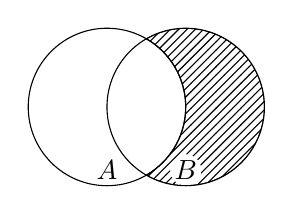
\begin{tikzpicture}
        \begin{scope}[even odd rule]
            \clip  (1,-0.8) circle (0.2) (1,0) circle (1);
            \filldraw [pattern = {north east lines}] (0.5,{0.5*sqrt(3)}) arc (60:-60:1) arc (-120:120:1);
        \end{scope}
        \draw (0,0) circle (1);
        \draw (1,0) circle (1);
        \draw (0,-0.8) node {$A$};
        \draw (1,-0.8) node {$B$};
    \end{tikzpicture}
\end{center}


关联目标:

暂未关联目标



标签: 第一单元

答案: $\{0, 2, 4\}$

解答或提示: 暂无解答与提示

使用记录:

20220510	2022届高三1班	\fcolorbox[rgb]{0,0,0}{1.000,0.000,0}{1.000}


出处: 赋能练习
\item { (000836)}已知集合$A=\{1,2,m\}$,$B=\{2,4\}$, 若$A\cup B=\{1,2,3,4\}$, 则实数$m=$\blank{50}.


关联目标:

暂未关联目标



标签: 第一单元

答案: $3$

解答或提示: 暂无解答与提示

使用记录:

20220525	2022届高三1班	\fcolorbox[rgb]{0,0,0}{1.000,0.000,0}{1.000}


出处: 赋能练习
\item { (000846)}已知全集$U=\mathbf{R}$,若集合$A=\{x|\dfrac x{x-1}>0\}$, 则$\complement_U A=$\blank{50}.


关联目标:

暂未关联目标



标签: 第一单元

答案: $[0,1]$

解答或提示: 暂无解答与提示

使用记录:

20220526	2022届高三1班	\fcolorbox[rgb]{0,0,0}{1.000,0.046,0}{0.977}


出处: 赋能练习
\item { (000857)}设集合$A=\{x||x|<2,\ x\in \mathbf{R}\}$, $B=\{x|x^2-4x+3\ge 0, \ x\in \mathbf{R}\}$, 则$A\cap B=$\blank{50}.


关联目标:

暂未关联目标



标签: 第一单元

答案: $(-2,1]$

解答或提示: 暂无解答与提示

使用记录:

20220527	2022届高三1班	\fcolorbox[rgb]{0,0,0}{1.000,0.094,0}{0.953}


出处: 赋能练习
\item { (000879)}若集合$A=\{x|3x+1>0\}$, $B=\{x||x-1|<2\}$, 则$A\cap B$=\blank{50}.


关联目标:

暂未关联目标



标签: 第一单元

答案: $(-\frac 13,3)$

解答或提示: 暂无解答与提示

使用记录:

20220602	2022届高三1班	\fcolorbox[rgb]{0,0,0}{1.000,0.094,0}{0.953}


出处: 赋能练习
\item { (000891)}已知集合$A=\{x||x-2|<a\}$, $B=\{x|x^2-2x-3<0\}$, 若$B\subseteq A$, 则实数$a$的取值范围是\blank{50}.


关联目标:

暂未关联目标



标签: 第一单元

答案: $a\ge 3$

解答或提示: 暂无解答与提示

使用记录:

20220607	2022届高三1班	\fcolorbox[rgb]{0,0,0}{1.000,0.372,0}{0.814}


出处: 赋能练习
\item { (000899)}设集合$M=\{x|x^2=x\}$, $N=\{x|\log_2 x\le 0\}$, 则$M\cup N=$\blank{50}.


关联目标:

暂未关联目标



标签: 第一单元

答案: $[0,1]$

解答或提示: 暂无解答与提示

使用记录:

20220613	2022届高三1班	\fcolorbox[rgb]{0,0,0}{1.000,0.418,0}{0.791}


出处: 赋能练习
\item { (000910)}若集合$A=\{x|y=\sqrt{x-1},\ x\in \mathbf{R}\}$, $B=\{x||x|\le 1,\ x\in \mathbf{R}\}$, 则$A\cap B=$\blank{50}.


关联目标:

暂未关联目标



标签: 第一单元

答案: $\{1\}$

解答或提示: 暂无解答与提示

使用记录:

20220615	2022届高三1班	\fcolorbox[rgb]{0,0,0}{1.000,0.046,0}{0.977}


出处: 赋能练习
\item { (000932)}集合$A=\{x|x^2-3x<0\}$, $B=\{x||x|<2\}$, 则$A\cup B$等于\blank{50}.


关联目标:

暂未关联目标



标签: 第一单元

答案: $(-2,3)$

解答或提示: 暂无解答与提示

使用记录:

20220622	2022届高三1班	\fcolorbox[rgb]{0,0,0}{1.000,0.094,0}{0.953}


出处: 赋能练习
\item { (000942)}已知集合$A=\{-1,3,2m-1\}$, 集合$B=\{3,m^2\}$. 若$B\subseteq A$, 则实数$m=$\blank{50}.


关联目标:

暂未关联目标



标签: 第一单元

答案: $1$

解答或提示: 暂无解答与提示

使用记录:

20220624	2022届高三1班	\fcolorbox[rgb]{0,0,0}{1.000,0.000,0}{1.000}


出处: 赋能练习
\item { (000964)}已知全集$U=\mathbf{R}$, 集合$A=\{x|(x-1)(x-4)\le 0\}$, 则集合$A$的补集$\complement_UA=$\blank{50}.


关联目标:

暂未关联目标



标签: 第一单元

答案: $(-\infty ,1)\cup (4,+\infty)$

解答或提示: 暂无解答与提示

使用记录:

20220629    2022届高三1班  	\fcolorbox[rgb]{0,0,0}{1.000,0.046,0}{0.977}


出处: 赋能练习
\item { (000989)}判断下列各组对象是否组成集合. (T or F)\\ 
\blank{30} (1) 大于$0$的偶数全体.\\ 
\blank{30} (2) 绝对值小于$0$的实数全体.\\ 
\blank{30} (3) 很小的数的全体.


关联目标:

暂未关联目标



标签: 第一单元

答案: 暂无答案

解答或提示: 暂无解答与提示

使用记录:

2016届11班	\fcolorbox[rgb]{0,0,0}{1.000,0.000,0}{1.000}	\fcolorbox[rgb]{0,0,0}{1.000,0.256,0}{0.872}	\fcolorbox[rgb]{0,0,0}{1.000,0.000,0}{1.000}

2016届12班	\fcolorbox[rgb]{0,0,0}{1.000,0.000,0}{1.000}	\fcolorbox[rgb]{0,0,0}{1.000,0.000,0}{1.000}	\fcolorbox[rgb]{0,0,0}{1.000,0.000,0}{1.000}


出处: 2016届创新班作业	1104-集合及其表示
\item { (000990)}用描述法或列举法(自行择其一种)表示下列集合.\\ 
(1) 大于$0$且小于$3$的实数的全体.\\ 
(2) 方程$x^3-x=0$的解的全体.\\ 
(3) 一次函数$y=2x+1$图像上所有点的全体.\\ 
(4) 被$3$除余$2$的整数的全体.


关联目标:

暂未关联目标



标签: 第一单元

答案: 暂无答案

解答或提示: 暂无解答与提示

使用记录:

2016届11班	\fcolorbox[rgb]{0,0,0}{1.000,0.102,0}{0.949}	\fcolorbox[rgb]{0,0,0}{1.000,0.102,0}{0.949}	\fcolorbox[rgb]{0,0,0}{1.000,0.000,0}{1.000}	\fcolorbox[rgb]{0,0,0}{1.000,0.462,0}{0.769}

2016届12班	\fcolorbox[rgb]{0,0,0}{1.000,0.052,0}{0.974}	\fcolorbox[rgb]{0,0,0}{1.000,0.154,0}{0.923}	\fcolorbox[rgb]{0,0,0}{1.000,0.052,0}{0.974}	\fcolorbox[rgb]{0,0,0}{1.000,0.564,0}{0.718}


出处: 2016届创新班作业	1104-集合及其表示
\item { (000991)}用列举法表示下列集合:\\ 
(1) $\left\{x\left| \dfrac{6}{3-x}\in\mathbf{Z},x\in\mathbf{Z}\right.\right\}$;\\ 
(2) $\{(x,y)|x+y=4,x,y\in\mathbf{N}\}$.


关联目标:

暂未关联目标



标签: 第一单元

答案: 暂无答案

解答或提示: 暂无解答与提示

使用记录:

2016届11班	\fcolorbox[rgb]{0,0,0}{1.000,0.512,0}{0.744}	\fcolorbox[rgb]{0,0,0}{1.000,0.000,0}{1.000}

2016届12班	\fcolorbox[rgb]{0,0,0}{1.000,0.564,0}{0.718}	\fcolorbox[rgb]{0,0,0}{1.000,0.102,0}{0.949}


出处: 2016届创新班作业	1104-集合及其表示
\item { (000992)}在直角坐标系中, 用图形表示下列集合:\\ 
(1) $\{(x,y)|\ 2<x<6,1<y<4,x,y\in\mathbf{R}\}$; \hfill (2) $\{(x,y)|\ 2<x<6,1<y<4,x,y\in\mathbf{Z}\}$.


关联目标:

暂未关联目标



标签: 第一单元

答案: 暂无答案

解答或提示: 暂无解答与提示

使用记录:

2016届11班	\fcolorbox[rgb]{0,0,0}{0.770,1.000,0}{0.385}	\fcolorbox[rgb]{0,0,0}{1.000,0.564,0}{0.718}

2016届12班	\fcolorbox[rgb]{0,0,0}{0.512,1.000,0}{0.256}	\fcolorbox[rgb]{0,0,0}{1.000,0.358,0}{0.821}


出处: 2016届创新班作业	1104-集合及其表示
\item { (000993)}集合$\left\{a,\dfrac{b}{a},1\right\}$和$\{0,a+b,a^2\}$ 表示同一个集合, 求实数$a,b$的值.


关联目标:

暂未关联目标



标签: 第一单元

答案: 暂无答案

解答或提示: 暂无解答与提示

使用记录:

2016届11班	\fcolorbox[rgb]{0,0,0}{1.000,0.358,0}{0.821}

2016届12班	\fcolorbox[rgb]{0,0,0}{1.000,0.564,0}{0.718}


出处: 2016届创新班作业	1104-集合及其表示
\item { (000994)}已知$a$是实数, 集合$M=\{x|\ ax^2+2x+a=0\}$有且仅有一个元素. 求满足上述条件的$a$所构成的集合.


关联目标:

暂未关联目标



标签: 第一单元

答案: 暂无答案

解答或提示: 暂无解答与提示

使用记录:

2016届11班	\fcolorbox[rgb]{0,0,0}{1.000,0.616,0}{0.692}

2016届12班	\fcolorbox[rgb]{0,0,0}{1.000,0.616,0}{0.692}


出处: 2016届创新班作业	1104-集合及其表示
\item { (000995)}已知非空集合$M$中的元素都是正整数, 且满足性质: 若$x\in M$, 则$4-x\in M$. 求满足条件的集合$M$.


关联目标:

暂未关联目标



标签: 第一单元

答案: 暂无答案

解答或提示: 暂无解答与提示

使用记录:

2016届11班	\fcolorbox[rgb]{0,0,0}{0.000,1.000,0}{0.000}

2016届12班	\fcolorbox[rgb]{0,0,0}{0.000,1.000,0}{0.000}


出处: 2016届创新班作业	1104-集合及其表示
\item { (000998)}满足$\{a_1,a_2\}\subseteq A\subsetneqq\{a_1,a_2,a_3,a_4,a_5,a_6\}$的集合$A$的个数是\blank{100}.


关联目标:

暂未关联目标



标签: 第一单元

答案: 暂无答案

解答或提示: 暂无解答与提示

使用记录:

2016届11班	\fcolorbox[rgb]{0,0,0}{1.000,0.206,0}{0.897}

2016届12班	\fcolorbox[rgb]{0,0,0}{1.000,0.422,0}{0.789}


出处: 2016届创新班作业	1105-集合的关系
\item { (001000)}设$A=\{n|\ n=3k+1,k \in \mathbf{Z}^+\}$, $B=\{n|\ n=3k-2,k \in \mathbf{Z}^+\}$.\\ 
(1) 集合$A$与集合$B$是相等的还是有真包含关系还是没有任何包含关系?\\ 
(2) 证明你的结论.


关联目标:

暂未关联目标



标签: 第一单元

答案: 暂无答案

解答或提示: 暂无解答与提示

使用记录:

2016届11班	\fcolorbox[rgb]{0,0,0}{1.000,0.000,0}{1.000}	\fcolorbox[rgb]{0,0,0}{1.000,0.358,0}{0.821}

2016届12班	\fcolorbox[rgb]{0,0,0}{1.000,0.052,0}{0.974}	\fcolorbox[rgb]{0,0,0}{1.000,0.474,0}{0.763}


出处: 2016届创新班作业	1105-集合的关系
\item { (001002)}设$a$是一个实数, 集合$A=\{x|\ x<2\}$, $B=\{x|\ x\leq a\}$, 且$A \subseteq B$.\\ 
(1) 实数$a$的取值范围为\blank{100};\\ 
(2) 试证明(1)的结论.


关联目标:

暂未关联目标



标签: 第一单元

答案: 暂无答案

解答或提示: 暂无解答与提示

使用记录:

2016届11班	\fcolorbox[rgb]{0,0,0}{1.000,0.052,0}{0.974}	\fcolorbox[rgb]{0,0,0}{0.410,1.000,0}{0.205}

2016届12班	\fcolorbox[rgb]{0,0,0}{1.000,0.000,0}{1.000}	\fcolorbox[rgb]{0,0,0}{0.000,1.000,0}{0.000}


出处: 2016届创新班作业	1105-集合的关系
\item { (001003)}已知集合$A=\{1,2\}$, $B=\{x|x^2-ax+a-1=0,\ x\in\mathbf{R}\}$, 若$B$不是$A$的真子集, 求实数$a$的值.


关联目标:

暂未关联目标



标签: 第一单元

答案: 暂无答案

解答或提示: 暂无解答与提示

使用记录:

2016届11班	\fcolorbox[rgb]{0,0,0}{1.000,0.974,0}{0.513}

2016届12班	\fcolorbox[rgb]{0,0,0}{1.000,0.894,0}{0.553}


出处: 2016届创新班作业	1105-集合的关系
\item { (001004)}设集合$A=\{1,-1\}$, $B=\{x|\ x^2-2ax+b=0,x\in\mathbf{R}\}$, 若$B\subseteq A$且$B\neq\varnothing$, 求实数$a,b$的值.


关联目标:

暂未关联目标



标签: 第一单元

答案: 暂无答案

解答或提示: 暂无解答与提示

使用记录:

2016届11班	\fcolorbox[rgb]{0,0,0}{1.000,0.256,0}{0.872}

2016届12班	\fcolorbox[rgb]{0,0,0}{1.000,0.368,0}{0.816}


出处: 2016届创新班作业	1105-集合的关系
\item { (001005)}设集合$A=\{x|x^2-x+a=0, x \in \mathbf{R}\}$, 求实数$a$的取值范围, 使得$A \subseteq \mathbf{R}^+$.


关联目标:

暂未关联目标



标签: 第一单元

答案: 暂无答案

解答或提示: 暂无解答与提示

使用记录:

2016届11班	\fcolorbox[rgb]{0,0,0}{0.512,1.000,0}{0.256}

2016届12班	\fcolorbox[rgb]{0,0,0}{0.894,1.000,0}{0.447}


出处: 2016届创新班作业	1105-集合的关系
\item { (001008)}已知集合$P\cap\{4,6\}=\{4\}$, $P\cap\{8,10\}=\{10\}$, $P\cap\{2,12\}=\{12\}$,
若$P\subseteq\{2,4,6,10,12\}$, 则$P=$\blank{50}.


关联目标:

暂未关联目标



标签: 第一单元

答案: 暂无答案

解答或提示: 暂无解答与提示

使用记录:

2016届11班	\fcolorbox[rgb]{0,0,0}{1.000,0.154,0}{0.923}

2016届12班	\fcolorbox[rgb]{0,0,0}{1.000,0.206,0}{0.897}


出处: 2016届创新班作业	1106-集合的运算
\item { (001010)}试用集合$A,B,C$的交, 并, 以及关于全集$U$的补运算表示下列文氏图所示的集合.
\begin{center}
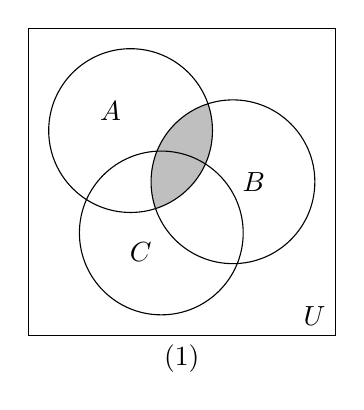
\begin{tikzpicture}[scale = 1.3]
    \begin{scope}
        \clip (1,2) circle (0.8);
        \clip (2,1.5) circle (0.8);     
        \fill [gray!50] (0,0) rectangle (3,3);
    \end{scope}
    \draw (1,2) circle (0.8) node [above left] {$A$};
    \draw (2,1.5) circle (0.8) node [right] {$B$};
    \draw (1.3,1) circle (0.8) node [below left] {$C$};
    \draw (3,0) node [above left] {$U$} rectangle (0,3);
    \draw (1.5,0) node [below] {(1)};   
\end{tikzpicture}
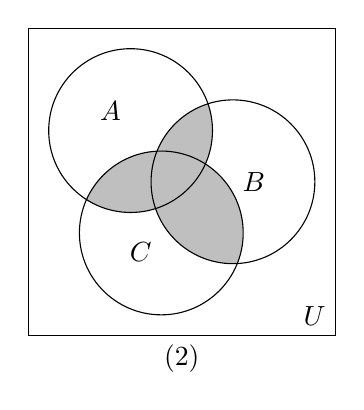
\begin{tikzpicture}[scale = 1.3]
    \begin{scope}
        \clip (1,2) circle (0.8);
        \clip (2,1.5) circle (0.8);     
        \fill [gray!50] (0,0) rectangle (3,3);
    \end{scope}
    \begin{scope}
        \clip (1.3,1) circle (0.8);
        \clip (2,1.5) circle (0.8);     
        \fill [gray!50] (0,0) rectangle (3,3);
    \end{scope}
    \begin{scope}
        \clip (1.3,1) circle (0.8);
        \clip (1,2) circle (0.8);     
        \fill [gray!50] (0,0) rectangle (3,3);
    \end{scope}
    \draw (1,2) circle (0.8) node [above left] {$A$};
    \draw (2,1.5) circle (0.8) node [right] {$B$};
    \draw (1.3,1) circle (0.8) node [below left] {$C$};
    \draw (3,0) node [above left] {$U$} rectangle (0,3);
    \draw (1.5,0) node [below] {(2)};   
\end{tikzpicture}
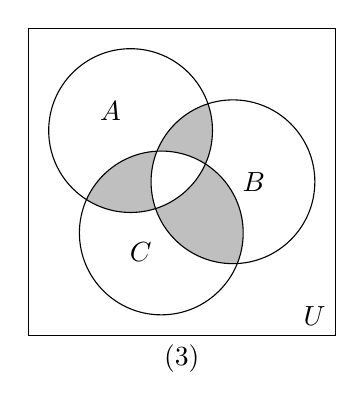
\begin{tikzpicture}[scale = 1.3]
    \begin{scope}[even odd rule]
        \clip (1,2) circle (0.8) (2,1.5) circle (0.8) (1.3,1) circle (0.8) (0,0) rectangle (3,3);
        \fill [gray!50] (1,2) circle (0.8);
        \fill [gray!50] (2,1.5) circle (0.8);
    \end{scope}
    \draw (1,2) circle (0.8) node [above left] {$A$};
    \draw (2,1.5) circle (0.8) node [right] {$B$};
    \draw (1.3,1) circle (0.8) node [below left] {$C$};
    \draw (3,0) node [above left] {$U$} rectangle (0,3);
    \draw (1.5,0) node [below] {(3)};   
\end{tikzpicture}
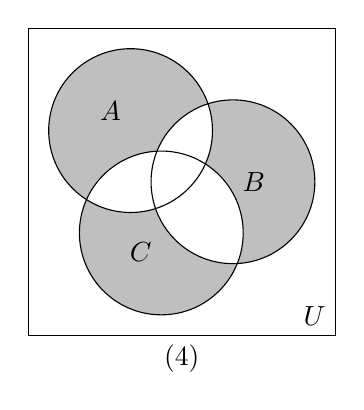
\begin{tikzpicture}[scale = 1.3]
    \begin{scope}[even odd rule]
        \clip (1,2) circle (0.8) (0,0) rectangle (3,3);
        \clip (2,1.5) circle (0.8) (0,0) rectangle (3,3);
        \fill [gray!50] (1.3,1) circle (0.8);
    \end{scope}
    \begin{scope}[even odd rule]
        \clip (1.3,1) circle (0.8) (0,0) rectangle (3,3);
        \clip (2,1.5) circle (0.8) (0,0) rectangle (3,3);
        \fill [gray!50] (1,2) circle (0.8);
    \end{scope}
    \begin{scope}[even odd rule]
        \clip (1,2) circle (0.8) (0,0) rectangle (3,3);
        \clip (1.3,1) circle (0.8) (0,0) rectangle (3,3);
        \fill [gray!50] (2,1.5) circle (0.8);
    \end{scope}
    \draw (1,2) circle (0.8) node [above left] {$A$};
    \draw (2,1.5) circle (0.8) node [right] {$B$};
    \draw (1.3,1) circle (0.8) node [below left] {$C$};
    \draw (3,0) node [above left] {$U$} rectangle (0,3);
    \draw (1.5,0) node [below] {(4)};   
\end{tikzpicture}
\end{center} 
1. \blank{200};2. \blank{200};\\ 
3. \blank{200};4. \blank{200}.


关联目标:

暂未关联目标



标签: 第一单元

答案: 暂无答案

解答或提示: 暂无解答与提示

使用记录:

2016届11班	\fcolorbox[rgb]{0,0,0}{1.000,0.000,0}{1.000}	\fcolorbox[rgb]{0,0,0}{1.000,0.102,0}{0.949}	\fcolorbox[rgb]{0,0,0}{1.000,0.666,0}{0.667}	\fcolorbox[rgb]{0,0,0}{1.000,0.564,0}{0.718}

2016届12班	\fcolorbox[rgb]{0,0,0}{1.000,0.000,0}{1.000}	\fcolorbox[rgb]{0,0,0}{1.000,0.052,0}{0.974}	\fcolorbox[rgb]{0,0,0}{1.000,0.974,0}{0.513}	\fcolorbox[rgb]{0,0,0}{1.000,0.820,0}{0.590}


出处: 2016届创新班作业	1106-集合的运算
\item { (001013)}已知集合$M=\{(x,y)|y=x+1, \ x \in \mathbf{R}\}$, $N=\{(x,y)|y=-x^2+4x,\  x \in \mathbf{R}\}$,
则$M \cap N=$\blank{80}.


关联目标:

暂未关联目标



标签: 第一单元

答案: 暂无答案

解答或提示: 暂无解答与提示

使用记录:

2016届11班	\fcolorbox[rgb]{0,0,0}{1.000,0.358,0}{0.821}

2016届12班	\fcolorbox[rgb]{0,0,0}{1.000,0.102,0}{0.949}


出处: 2016届创新班作业	1106-集合的运算
\item { (001014)}已知集合$M=\{y|y=x+1, \ x \in \mathbf{R}\}$, $N=\{y|y=-x^2+4x,\  x \in \mathbf{R}\}$,
则$M \cap N=$\blank{80}.


关联目标:

暂未关联目标



标签: 第一单元

答案: 暂无答案

解答或提示: 暂无解答与提示

使用记录:

2016届11班	\fcolorbox[rgb]{0,0,0}{0.820,1.000,0}{0.410}

2016届12班	\fcolorbox[rgb]{0,0,0}{0.616,1.000,0}{0.308}


出处: 2016届创新班作业	1106-集合的运算
\item { (001015)}已知集合$A=\{x|\ x^2+px+q=0\}$, $B=\{x|\ x^2-x+r=0\}$, 且$A\cap B=\{-1\}$, $A\cup B=\{-1,2\}$, 求实数$p,q,r$的值.


关联目标:

暂未关联目标



标签: 第一单元

答案: 暂无答案

解答或提示: 暂无解答与提示

使用记录:

2016届11班	\fcolorbox[rgb]{0,0,0}{1.000,0.666,0}{0.667}

2016届12班	\fcolorbox[rgb]{0,0,0}{1.000,0.820,0}{0.590}


出处: 2016届创新班作业	1106-集合的运算
\item { (001016)}已知集合$A=\{1,2\}$, $B=\{x|mx^2+2mx-1<0, x \in\mathbf{R}\}$. 已知$A \cap B=\{1\}$, 求实数$m$的取值范围.


关联目标:

暂未关联目标



标签: 第一单元

答案: 暂无答案

解答或提示: 暂无解答与提示

使用记录:

2016届11班	\fcolorbox[rgb]{0,0,0}{1.000,0.410,0}{0.795}

2016届12班	\fcolorbox[rgb]{0,0,0}{1.000,0.616,0}{0.692}


出处: 2016届创新班作业	1106-集合的运算
\item { (001017)}设$A,B$是两个集合, 求证: ``$A\cap B=A$''当且仅当``$A \subseteq B$''.(用文氏图画一下并不算证明)


关联目标:

暂未关联目标



标签: 第一单元

答案: 暂无答案

解答或提示: 暂无解答与提示

使用记录:

2016届11班	\fcolorbox[rgb]{0,0,0}{0.512,1.000,0}{0.256}

2016届12班	\fcolorbox[rgb]{0,0,0}{0.358,1.000,0}{0.179}


出处: 2016届创新班作业	1106-集合的运算
\item { (001029)}设$f(x)$是$m$次多项式, $g(x)$是$n$次多项式, $m,n$均为正整数. 判断下列命题的真假(T or F).\\ 
\blank{30} (1) 多项式$-2f(x)$的次数为$m$;\\ 
\blank{30} (2) 多项式$f(x)+g(x)$的次数为$\max\{m,n\}$($\max$表示集合中较大的那个数);\\ 
\blank{30} (3) 多项式$f(x)\times g(x)$的次数为$m+n$;\\ 
\blank{30} (4) 多项式$[f(x)]^2+f(x)+1$的次数为$2m$;


关联目标:

暂未关联目标



标签: 第一单元

答案: 暂无答案

解答或提示: 暂无解答与提示

使用记录:

2016届11班	\fcolorbox[rgb]{0,0,0}{1.000,0.000,0}{1.000}	\fcolorbox[rgb]{0,0,0}{1.000,0.462,0}{0.769}	\fcolorbox[rgb]{0,0,0}{1.000,0.102,0}{0.949}	\fcolorbox[rgb]{0,0,0}{1.000,0.102,0}{0.949}

2016届12班	\fcolorbox[rgb]{0,0,0}{1.000,0.000,0}{1.000}	\fcolorbox[rgb]{0,0,0}{1.000,0.512,0}{0.744}	\fcolorbox[rgb]{0,0,0}{1.000,0.000,0}{1.000}	\fcolorbox[rgb]{0,0,0}{1.000,0.102,0}{0.949}


出处: 2016届创新班作业	1110-多项式的有关概念
\item { (002693)}已知$P=\{y=x^2+1\}$, $Q=\{y|y=x^2+1, \ x\in \mathbf{R}\}$, $E=\{x|y=x^2+1, \  x\in \mathbf{R}\}$, $F=\{(x,y)|y=x^2+1, \ x\in \mathbf{R}\}$, $G=\{x|x\ge 1\}$, $H=\{x|x^2+1=0, \ x\in \mathbf{R}\}$, 则各集合间关系正确的有\blank{50}. (答案可能不唯一)\\
\textcircled{1} $P=F$; \textcircled{2} $Q=E$; \textcircled{3} $E=F$; \textcircled{4} $Q\subseteq G$; \textcircled{5} $H\subsetneqq P$


关联目标:

暂未关联目标



标签: 第一单元

答案: 暂无答案

解答或提示: 暂无解答与提示

使用记录:

暂无使用记录


出处: 2022届高三第一轮复习讲义
\item { (002697)}设全集$U=\{2,3,a^2+2a-3\}$, 集合$A=\{|2a-1|,2\}$, $\complement_U A=\{5\}$, 则实数$a=$\blank{50}.


关联目标:

暂未关联目标



标签: 第一单元

答案: 暂无答案

解答或提示: 暂无解答与提示

使用记录:

暂无使用记录


出处: 2022届高三第一轮复习讲义
\item { (002700)}集合$C=\{x|x=\dfrac k2\pm \dfrac14, \ k\in \mathbf{Z}\},D=\{x|x=\dfrac k4,\ k\in \mathbf{Z}\}$, 试判断$C$与$D$的关系, 并证明.


关联目标:

暂未关联目标



标签: 第一单元

答案: 暂无答案

解答或提示: 暂无解答与提示

使用记录:

暂无使用记录


出处: 2022届高三第一轮复习讲义
\item { (002701)}集合$A=\{x|x^2+4x=0\}$, $B=\{x|x^2+2(a+1)x+a^2-1=0,\ x\in \mathbf{R}\}$.\\
(1) 若$A\cap B=A$, 求实数$a$的取值范围;\\
(2) 若$A\cup B=A$, 求实数$a$的取值范围.


关联目标:

暂未关联目标



标签: 第一单元

答案: 暂无答案

解答或提示: 暂无解答与提示

使用记录:

暂无使用记录


出处: 2022届高三第一轮复习讲义
\item { (002702)}若集合$A=[2,3]$, 集合$B=[a,2a+1]$.\\
(1) 若$A\subsetneqq B$, 求实数$a$的取值范围;\\
(2) 若$A\cap B\ne \varnothing$, 求实数$a$的取值范围.


关联目标:

暂未关联目标



标签: 第一单元

答案: 暂无答案

解答或提示: 暂无解答与提示

使用记录:

暂无使用记录


出处: 2022届高三第一轮复习讲义
\item { (002703)}设全集$U=\mathbf{R}$, 函数$y=f(x)$, $y=g(x)$, $y=h(x)$的定义域均为$\mathbf{R}$. 设集合$A=\{x|f(x)=0\}$, $B=\{x|g(x)=0\}$, $C=\{x|h(x)=0, \ x\in \mathbf{R}\}$, 则方程$\dfrac{f^2(x)+g^2(x)}{h(x)}=0$的解集是\blank{50}(用$U,A,B,C$表示).


关联目标:

暂未关联目标



标签: 第一单元

答案: 暂无答案

解答或提示: 暂无解答与提示

使用记录:

暂无使用记录


出处: 2022届高三第一轮复习讲义
\item { (002704)}(1) 已知集合$A=\{y|y=x^2, \ x\in \mathbf{R}\}, B=\{y|y=4-x^2, \ x\in \mathbf{R}\}$, 则$A\cap B=$\blank{50}.\\
(2) 已知集合$A=\{(x,y)|y={x^2},\ x\in \mathbf{R}\}$, $B=\{(x,y)|y=4-x^2, \ x\in \mathbf{R}\}$, 则$A\cap B=$\blank{50}.


关联目标:

暂未关联目标



标签: 第一单元

答案: 暂无答案

解答或提示: 暂无解答与提示

使用记录:

暂无使用记录


出处: 2022届高三第一轮复习讲义
\item { (002706)}(1) 集合$A$满足$\{1\}\subseteq A \subsetneqq \{1,2,3,4\}$, 则满足条件的集合$A$有\blank{50}个.
(2) 若$A\cup B=\{1,2\}$, 将满足条件的集合$A$, $B$写成有序集合对$(A,B)$, 则有序集合对$(A,B)$有\blank{50}个.


关联目标:

暂未关联目标



标签: 第一单元

答案: 暂无答案

解答或提示: 暂无解答与提示

使用记录:

暂无使用记录


出处: 2022届高三第一轮复习讲义
\item { (002708)}设集合$A=\{x|x^2+px+1=0,\ x\in \mathbf{R}\}$, 若$A\cap \mathbf{R}^+=\varnothing$. 求实数p的取值范围.


关联目标:

暂未关联目标



标签: 第一单元

答案: 暂无答案

解答或提示: 暂无解答与提示

使用记录:

暂无使用记录


出处: 2022届高三第一轮复习讲义
\item { (002709)}设函数$f(x)=\lg (\dfrac2{x+1}-1)$的定义域为集合$A$, 函数$g(x)=\sqrt{1-|x+a|}$的定义域为集合$B$.\\
(1) 当$a=1$时, 求集合$B$.\\
(2) 问: $a\ge 2$是$A\cap B=\varnothing$的什么条件(在``充分非必要条件、必要非充分条件、充要条件、既非充分也非必要条件''中选一)?并证明你的结论.


关联目标:

暂未关联目标



标签: 第一单元

答案: 暂无答案

解答或提示: 暂无解答与提示

使用记录:

暂无使用记录


出处: 2022届高三第一轮复习讲义
\item { (002710)}如图, $U$为全集, $M,P,S$是$U$的三个子集, 则阴影部分所表示的集合是\bracket{20}.
\begin{center}
    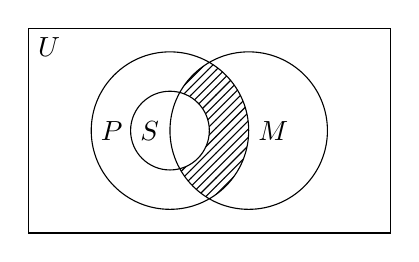
\begin{tikzpicture}
        \begin{scope}
            \clip (1,0) circle (1);
            \begin{scope}[even odd rule]
                \clip (0,0) circle (1) (0,0) circle (0.5);
                \filldraw [pattern = {north east lines}] (-2,-2) rectangle (2,2);
            \end{scope}
        \end{scope}
        \draw (0,0) circle (1) (1,0) circle (1) (0,0) circle (0.5);
        \draw (-1.8,-1.3) rectangle (2.8,1.3);
        \draw (-1.8,1.3) node [below right] {$U$} (-1,0) node [right] {$P$} (-0.5,0) node [right] {$S$} (1,0) node [right] {$M$};
    \end{tikzpicture}
\end{center}
\fourch{$(M\cap P)\cap S$}{$(M\cap P)\cup S$}{$(M\cap P)\cap \complement_U S$}{$(M\cap P)\cup \complement_U S$}


关联目标:

暂未关联目标



标签: 第一单元

答案: 暂无答案

解答或提示: 暂无解答与提示

使用记录:

暂无使用记录


出处: 2022届高三第一轮复习讲义
\item { (002711)}设集合$A=\{5,\log_2(a+3)\}$, $B=\{a,b\}$, 若$A\cap B=\{2\}$, 则$A\cup B=$\blank{50}.


关联目标:

暂未关联目标



标签: 第一单元

答案: 暂无答案

解答或提示: 暂无解答与提示

使用记录:

暂无使用记录


出处: 2022届高三第一轮复习讲义
\item { (002712)}设集合$A\cap \{-2,0,1\}=\{0,1\}$, $A\cup \{-2,0,2\}=\{-2,0,1,2\}$, 则满足上述条件的集合$A$的个数为\blank{50}个.


关联目标:

暂未关联目标



标签: 第一单元

答案: 暂无答案

解答或提示: 暂无解答与提示

使用记录:

暂无使用记录


出处: 2022届高三第一轮复习讲义
\item { (002713)}若集合$A=\{x|x\le 2\}$, $B=\{x|x\ge a\}$, 满足$A\cap B=\{2\}$, 则实数$a=$\blank{50}.


关联目标:

暂未关联目标



标签: 第一单元

答案: 暂无答案

解答或提示: 暂无解答与提示

使用记录:

暂无使用记录


出处: 2022届高三第一轮复习讲义
\item { (002714)}若集合$M=[a-1,a+1]$, $N=(-\infty,-1)\cup [2,+\infty)$, 且$M\cap N=\varnothing$, 则实数$a$的取值范围为\blank{50}.


关联目标:

暂未关联目标



标签: 第一单元

答案: 暂无答案

解答或提示: 暂无解答与提示

使用记录:

暂无使用记录


出处: 2022届高三第一轮复习讲义
\item { (002715)}集合$A=\{(x,y)|x^2+y^2=25\}$, $B=\{(x,y)|x=3y=4\}$, 则$A\cap B$的子集个数是\blank{50}个.


关联目标:

暂未关联目标



标签: 第一单元

答案: 暂无答案

解答或提示: 暂无解答与提示

使用记录:

暂无使用记录


出处: 2022届高三第一轮复习讲义
\item { (002716)}已知集合$M=\{x|x=3m+1, \ m\in \mathbf{Z}\}$, $N=\{y|y=3m+2, \ m\in \mathbf{Z}\}$, 若$x_0\in M$, $y_0\in N$, 则$x_0y_0$与集合$M,N$的关系是\bracket{20}.
\twoch{$x_0y_0\in M$但$x_0y_0$$\notin N$}{$x_0y_0\in N$但$x_0y_0\notin M$}{$x_0y_0\notin M$且$x_0y_0\notin N$}{$x_0y_0$$\in M$且$x_0y_0\in N$}


关联目标:

暂未关联目标



标签: 第一单元

答案: 暂无答案

解答或提示: 暂无解答与提示

使用记录:

暂无使用记录


出处: 2022届高三第一轮复习讲义
\item { (002718)}设常数$a\in \mathbf{R}$, 集合$A=\{x|\dfrac{3-2x}{x-1}+1 \ge 0, \ x\in \mathbf{R}\}$, $B=\{x|2ax<a+x, \ x\in \mathbf{R} \}$.若$A\cup B=B$, 求$a$的取值范围.


关联目标:

暂未关联目标



标签: 第一单元

答案: 暂无答案

解答或提示: 暂无解答与提示

使用记录:

暂无使用记录


出处: 2022届高三第一轮复习讲义
\item { (002720)}设常数$k\in \mathbf{R}$, 关于$x$的不等式组$\begin{cases} x^2-x-2>0, \\ 2x^2+(2k+5)x+5k<0 \end{cases}$ 整数解的集合为$\{-2\}$, 求实数$k$的取值范围.


关联目标:

暂未关联目标



标签: 第一单元

答案: 暂无答案

解答或提示: 暂无解答与提示

使用记录:

暂无使用记录


出处: 2022届高三第一轮复习讲义
\item { (002723)}定义集合运算: $A\odot B=\{z|z=xy(x+y), \ x\in A, \ y\in B \}$, 设集合$A=\{0,1\}$, $B=\{2,3\}$, 则集合$A\odot B$的所有元素之和为\blank{50}.


关联目标:

暂未关联目标



标签: 第一单元

答案: 暂无答案

解答或提示: 暂无解答与提示

使用记录:

暂无使用记录


出处: 2022届高三第一轮复习讲义
\item { (002725)}集合$A=\{(x,y)|y=|x|+1\}$, $B=\{(x,y)|y=\dfrac12x+a\}$, 若$A\cap B=\varnothing$, 则$a$的取值范围是\blank{50}.


关联目标:

暂未关联目标



标签: 第一单元

答案: 暂无答案

解答或提示: 暂无解答与提示

使用记录:

暂无使用记录


出处: 2022届高三第一轮复习讲义
\item { (002727)}已知集合$A=\{x|ax^2-3x+2=0\}$至多有一个元素, 则$a$的取值范围是\blank{50}; 若至少有一个元素, 则$a$的取值范围是\blank{50}.


关联目标:

暂未关联目标



标签: 第一单元

答案: 暂无答案

解答或提示: 暂无解答与提示

使用记录:

暂无使用记录


出处: 2022届高三第一轮复习讲义
\item { (002728)}设含有三个实数的集合既可以表示为$\{a,\dfrac ba,1\}$, 又可以表示为$\{a^2,a+b,0\}$, 那么$a+b=$\blank{50}.


关联目标:

暂未关联目标



标签: 第一单元

答案: 暂无答案

解答或提示: 暂无解答与提示

使用记录:

暂无使用记录


出处: 2022届高三第一轮复习讲义
\item { (002729)}设$f(x)=x^2-12x+36$, $A=\{a|1\le a\le 10, \ a\in \mathbf{N}\}$, $B=\{b|b=f(a),\ a\in A\}$, 又设$C=A\cap B$. 求集合$C$.


关联目标:

暂未关联目标



标签: 第一单元

答案: 暂无答案

解答或提示: 暂无解答与提示

使用记录:

暂无使用记录


出处: 2022届高三第一轮复习讲义
\item { (002807)}已知关于$x$的不等式$\dfrac{ax-5}{x^2-a}<0$的解集为$M$.\\
(1) 当$a=5$时, 求集合$M$;\\
(2) 若$2\in M$且$5\notin M$, 求实数$a$的取值范围.


关联目标:

暂未关联目标



标签: 第一单元

答案: 暂无答案

解答或提示: 暂无解答与提示

使用记录:

暂无使用记录


出处: 2022届高三第一轮复习讲义
\item { (003610)}已知集合$A=\{1,2,4\}$,$B=\{2,4,5\}$, 则$A\cap B=$\blank{50}.


关联目标:

暂未关联目标



标签: 第一单元

答案: 暂无答案

解答或提示: 暂无解答与提示

使用记录:

暂无使用记录


出处: 上海2020年秋季高考试题1
\item { (003631)}已知集合$A=(-\infty,3)$, $B=(2,+\infty)$, 则$A\cap B=$\blank{50}.


关联目标:

暂未关联目标



标签: 第一单元

答案: 暂无答案

解答或提示: 暂无解答与提示

使用记录:

暂无使用记录


出处: 上海2019年秋季高考试题1
\item { (003673)}已知集合$A=\{1,2,3,4\}$, $B=\{3,4,5\}$, 则$A\cap B=$\blank{50}.


关联目标:

暂未关联目标



标签: 第一单元

答案: 暂无答案

解答或提示: 暂无解答与提示

使用记录:

暂无使用记录


出处: 上海2017年秋季高考试题1
\item { (003695)}设实数$a,b,c$满足: $ac\ne 0$且$a\ne c$, 集合$A=\{y|y=ax^2+bx+c, \ x\in \mathbf{R}\}$, $B=\{y|y=cx^2+bx+a\}$, 以下结论一定正确的是\bracket{20}.
\fourch{$A\subseteq B$}{$B\subseteq A$}{$A\cup B=\mathbf{R}$}{$A\cap B\ne\varnothing$}


关联目标:

暂未关联目标



标签: 第一单元

答案: 暂无答案

解答或提示: 暂无解答与提示

使用记录:

暂无使用记录


出处: 2022届高三高考前冲刺题精选
\item { (003707)}若全集$U=\{x|x^2-7x+12\le 0\}$, 集合$M=\{x|3<x<4\}$, $N=\left\{x\left|\dfrac{x-3}{4-x}\ge 0\right.\right\}$, 则$\complement_U M\cap \complement_U N=$\blank{50}.


关联目标:

暂未关联目标



标签: 第一单元

答案: 暂无答案

解答或提示: 暂无解答与提示

使用记录:

暂无使用记录


出处: 2016年双基百分百
\item { (003719)}若集合$A=\{x|x^2-2x<0\}$, $B=\{x||x|<1\}$, 则$A\cup B$等于\blank{50}.


关联目标:

暂未关联目标



标签: 第一单元

答案: 暂无答案

解答或提示: 暂无解答与提示

使用记录:

暂无使用记录


出处: 2016年双基百分百
\item { (003745)}已知集合$A=\{y|y=\sin x, \ x\in \mathbf{R}\}$, $B=\{x|x(2-x)>0\}$, 则$A\cup B=$\blank{50}.


关联目标:

暂未关联目标



标签: 第一单元|第三单元

答案: 暂无答案

解答或提示: 暂无解答与提示

使用记录:

暂无使用记录


出处: 2016年双基百分百
\item { (003760)}已知集合$A=\{1,3,\sqrt{m}\}$, $B=\{1,m\}$, $A\cup B=A$, 则$m=$\blank{50}.


关联目标:

暂未关联目标



标签: 第一单元

答案: 暂无答案

解答或提示: 暂无解答与提示

使用记录:

暂无使用记录


出处: 2016年双基百分百
\item { (003774)}已知集合$A=\left\{x\left|\dfrac{2x+1}{x+2}<1, \ x\in \mathbf{R}\right.\right\}$, 函数$f(x)=|mx+1| \ (m\in \mathbf{R})$. 函数$g(x)=x^2+ax+b \ (a,b\in \mathbf{R})$的值域为$[0,+\infty)$.\\
(1) 若不等式$f(x)<3$的解集为$A$, 求$m$的值;\\
(2) 在(1)的条件下, 若$\left|f(x)-2f\left(\dfrac x 2\right)\right|\le k$恒成立, 求$k$的取值范围;\\
(3) 若关于$x$的不等式$g(x)<c$的解集为$(m,m+6)$, 求实数$c$的值.


关联目标:

暂未关联目标



标签: 第一单元

答案: 暂无答案

解答或提示: 暂无解答与提示

使用记录:

暂无使用记录


出处: 2016年双基百分百
\item { (003835)}若集合$A=\{x||x-2|\le 2\}$, $B=\{y|y=-x^2, \ -1\le x\le 2\}$, 则$A\cap B=$\blank{50}.


关联目标:

暂未关联目标



标签: 第一单元

答案: 暂无答案

解答或提示: 暂无解答与提示

使用记录:

暂无使用记录


出处: 2016年双基百分百
\item { (003860)}若集合$M=\{y|y=x^2-1, \ x\in \mathbf{R}\}$, 集合$N=\{x|y=\sqrt{3-x}, \ x\in \mathbf{R}\}$, 则$M\cap N=$\blank{30}.
\fourch{$\{(-\sqrt{2},1),(\sqrt{2},1)\}$}{$\{t|0\le t\le \sqrt{3}\}$}{$\{t|-1\le t\le 3\}$}{$\{t|-\infty<t\le \sqrt{3}\}$}


关联目标:

暂未关联目标



标签: 第一单元

答案: 暂无答案

解答或提示: 暂无解答与提示

使用记录:

暂无使用记录


出处: 2016年双基百分百
\item { (003925)}已知集合$A=\{x|x^2-2x\le 0 \}$, $B=\{x|-1<x<1\}$, 则$A\cap B=$\blank{50}.


关联目标:

暂未关联目标



标签: 第一单元

答案: 暂无答案

解答或提示: 暂无解答与提示

使用记录:

暂无使用记录


出处: 2016年双基百分百
\item { (003957)}已知集合$P=\{a,-1\}$, $Q=\{x|x^2-1<0, \ x\in \mathbf{Z}\}$, 如果$P\cap Q\ne\varnothing$, 则实数$a=$\blank{50}.


关联目标:

暂未关联目标



标签: 第一单元

答案: 暂无答案

解答或提示: 暂无解答与提示

使用记录:

暂无使用记录


出处: 2016年双基百分百
\item { (004059)}已知集合$A=\{-2,1,2\}$, $B=\{\sqrt a+1,a\}$, 且$B\subseteq A$, 则实数$a$的值是\blank{50}.


关联目标:

暂未关联目标



标签: 第一单元

答案: $1$

解答或提示: 暂无解答与提示

使用记录:

20220301	2022届高三1班	\fcolorbox[rgb]{0,0,0}{1.000,0.000,0}{1.000}


出处: 2022届高三下学期测验卷01第1题
\item { (004080)}集合$A=\{1,2,3,4\}$, $B=\{x|(x-1)(x-5)<0\}$, 则$A\cap B=$\blank{50}.


关联目标:

暂未关联目标



标签: 第一单元

答案: 暂无答案

解答或提示: 暂无解答与提示

使用记录:

20220308	2022届高三1班	\fcolorbox[rgb]{0,0,0}{1.000,0.046,0}{0.977}


出处: 2022届高三下学期测验卷02第1题
\item { (004123)}设集合$A=\{1,2,3\}$, $B=\{y|y=\sin x, \ x\in \mathbf{R}\}$, 则$A\cap B=$\blank{50}.


关联目标:

暂未关联目标



标签: 第一单元

答案: 暂无答案

解答或提示: 暂无解答与提示

使用记录:

20220331	2022届高三1班	\fcolorbox[rgb]{0,0,0}{1.000,0.000,0}{1.000}


出处: 2022届高三下学期测验卷04第2题
\item { (004144)}已知集合$M=\{x||x+1|\le 1\}$, $N=\{-1,0,1\}$, 则$M\cap N=$\blank{50}.


关联目标:

暂未关联目标



标签: 第一单元

答案: 暂无答案

解答或提示: 暂无解答与提示

使用记录:

20220407	2022届高三1班	\fcolorbox[rgb]{0,0,0}{1.000,0.094,0}{0.953}


出处: 2022届高三下学期测验卷05第2题
\item { (004164)}集合$A=\{x|x^2-2x<0\}$, $B=\{x||x|<1\}$, 则$A\cup B$=\blank{50}.


关联目标:

暂未关联目标



标签: 第一单元

答案: 暂无答案

解答或提示: 暂无解答与提示

使用记录:

20220421	2022届高三1班	\fcolorbox[rgb]{0,0,0}{1.000,0.140,0}{0.930}


出处: 2022届高三下学期测验卷06第1题
\item { (004227)}已知集合$A=\{1,3,m\}$, $B=\{3,5\}$, 且$B\subseteq A$, 则实数$m$的值是\blank{50}.


关联目标:

暂未关联目标



标签: 第一单元

答案: 暂无答案

解答或提示: 暂无解答与提示

使用记录:

20220512	2022届高三1班	\fcolorbox[rgb]{0,0,0}{1.000,0.000,0}{1.000}


出处: 2022届高三下学期测验卷09第1题
\item { (004271)}若集合$A=\{2,4,6,8\}$, $B=\{x|x^2-4x\le 0\}$, 则$A\cap B=$\blank{50}.


关联目标:

暂未关联目标



标签: 第一单元

答案: 暂无答案

解答或提示: 暂无解答与提示

使用记录:

20220524	2022届高三1班	\fcolorbox[rgb]{0,0,0}{1.000,0.000,0}{1.000}


出处: 2022届高三下学期测验卷11第3题
\item { (004292)}已知集合$P=\{x|(x+1)(x–3)<0\}$, $Q=\{x||x|>2\}$, 则$P\cap Q=$\blank{50}.


关联目标:

暂未关联目标



标签: 第一单元

答案: 暂无答案

解答或提示: 暂无解答与提示

使用记录:

20220607	2022届高三1班	\fcolorbox[rgb]{0,0,0}{1.000,0.094,0}{0.953}


出处: 2022届高三下学期测验卷12第3题
\item { (004311)}设$m\in \mathbf{R}$. 已知集合$A=\{2,3\}$, $B=\{1,m\}$. 若$4-m\in A$, 则$m=$\blank{50}.


关联目标:

暂未关联目标



标签: 第一单元

答案: 暂无答案

解答或提示: 暂无解答与提示

使用记录:

20220627	2022届高三1班	\fcolorbox[rgb]{0,0,0}{1.000,0.000,0}{1.000}


出处: 2022届高三下学期测验卷13第1题
\item { (004353)}已知全集$U=\{x|x<2\}$, 集合$A=\{x|x<1\}$, 则$\complement_UA=$\blank{50}.


关联目标:

暂未关联目标



标签: 第一单元

答案: 暂无答案

解答或提示: 暂无解答与提示

使用记录:

20210918	2022届高三1班	\fcolorbox[rgb]{0,0,0}{1.000,0.046,0}{0.977}


出处: 2022届高三上学期测验卷01第1题
\item { (004354)}设集合$A=\{x||x-2|<1, \ x\in\mathbf{R}\}$, $B=\{x|\dfrac{x-3}{x-1}\ge 0\}$, 则$A\cup B=$\blank{50}.


关联目标:

暂未关联目标



标签: 第一单元

答案: 暂无答案

解答或提示: 暂无解答与提示

使用记录:

20210918	2022届高三1班	\fcolorbox[rgb]{0,0,0}{1.000,0.140,0}{0.930}


出处: 2022届高三上学期测验卷01第2题
\item { (004374)}设集合$A=\{1,2,3\}$, $B=\{x|x<3\}$, 则$A\cap B=$\blank{50}.


关联目标:

暂未关联目标



标签: 第一单元

答案: 暂无答案

解答或提示: 暂无解答与提示

使用记录:

20210928	2022届高三1班	\fcolorbox[rgb]{0,0,0}{1.000,0.000,0}{1.000}


出处: 2022届高三上学期测验卷02第1题
\item { (004382)}已知常数$m,n\in \mathbf{Z}$, 若对任意$x\in [0,+\infty)$, 不等式$(mx-2)(x^2-2n)\ge 0$恒成立, 则$m+n$的取值集合为\blank{50}.


关联目标:

暂未关联目标



标签: 第一单元

答案: 暂无答案

解答或提示: 暂无解答与提示

使用记录:

20210928	2022届高三1班	\fcolorbox[rgb]{0,0,0}{1.000,0.326,0}{0.837}


出处: 2022届高三上学期测验卷02第9题
\item { (004403)}设集合$A=\{y|y=a^x,\ x>0\}$(其中常数$a>0,  \ a\ne 1$), $B=\{y|y=x^k,\ x\in A\}$(其中常数$k\in \mathbf{Q}$), 则``$k<0$''是``$A\cap B=\varnothing$''的\bracket{20}.
\twoch{充分非必要条件}{必要非充分条件}{充分必要条件}{既非充分又非必要条件}


关联目标:

暂未关联目标



标签: 第一单元|第二单元

答案: 暂无答案

解答或提示: 暂无解答与提示

使用记录:

20211012	2022届高三1班	\fcolorbox[rgb]{0,0,0}{1.000,0.954,0}{0.523}


出处: 2022届高三上学期测验卷03第16题
\item { (004414)}已知集合$M=\{y|y=3\sin x,x\in \mathbf{R}\}$, $N=\{x||x|<a\}$, 若$M\subseteq N$, 则实数$a$的取值范围是\blank{50}.


关联目标:

暂未关联目标



标签: 第一单元

答案: 暂无答案

解答或提示: 暂无解答与提示

使用记录:

20211018	2022届高三1班	\fcolorbox[rgb]{0,0,0}{1.000,0.142,0}{0.929}


出处: 2022届高三上学期测验卷04第6题
\item { (004421)}已知$M$、$N$、$P\subseteq \mathbf{R}$, $M=\{x|f(x)=0\}$, $N=\{x|g(x)=0\}$, $P=\{x|f(x)g(x)=0\}$, 则集合$P$恒满足的关系为\bracket{20}.
\fourch{$P=M\cup N$}{$P\ne \varnothing$}{$P=\varnothing$}{$P\subseteq (M\cup N)$}


关联目标:

暂未关联目标



标签: 第一单元

答案: 暂无答案

解答或提示: 暂无解答与提示

使用记录:

20211018	2022届高三1班	\fcolorbox[rgb]{0,0,0}{1.000,0.238,0}{0.881}


出处: 2022届高三上学期测验卷04第13题
\item { (004422)}已知$a_1$、$a_2$与$b_1$、$b_2$是$4$个不同的实数, 关于x的方程$|x-a_1|+|x-a_2|=|x-b_1|+|x-b_2|$的解集为$A$, 则集合$A$中元素的个数为\bracket{20}.
\twoch{$1$个}{$0$个或$1$个或$2$个}{$0$个或$1$个或$2$个或无限个}{$1$个或无限个}


关联目标:

暂未关联目标



标签: 第一单元|第二单元

答案: 暂无答案

解答或提示: 暂无解答与提示

使用记录:

20211018	2022届高三1班	\fcolorbox[rgb]{0,0,0}{0.952,1.000,0}{0.476}


出处: 2022届高三上学期测验卷04第14题
\item { (004435)}集合$A=\{y|y=\log_{\frac 12}x-x,1\le x\le 2\}$, $B=\{x|x^2-5tx+1\le 0\}$, 若$A\cap B=A$, 则实数$t$的取值范围是\blank{50}.


关联目标:

暂未关联目标



标签: 第一单元|第二单元

答案: 暂无答案

解答或提示: 暂无解答与提示

使用记录:

20211026	2022届高三1班	\fcolorbox[rgb]{0,0,0}{1.000,0.326,0}{0.837}


出处: 2022届高三上学期测验卷05第11题
\item { (004468)}设全集$U=\mathbf{R}$集合$A=\{-2,-1,0,1,2\}$, $B=\{x|x\ge 0\}$, 则$A\cap \complement_UB=$\blank{50}.


关联目标:

暂未关联目标



标签: 第一单元

答案: 暂无答案

解答或提示: 暂无解答与提示

使用记录:

20211116	2022届高三1班	\fcolorbox[rgb]{0,0,0}{1.000,0.000,0}{1.000}


出处: 2022届高三上学期测验卷07第2题
\item { (004499)}已知集合$M=\{1,2,3,\cdots,10\}$, 集合$A\subseteq M$, 定义$M(A)$为$A$中元素的最大值, 当$A$取遍$M$的所有非空子集时, 对应的$M(A)$的和记为$S_{10}$, 则$S_{10}=$\blank{50}.


关联目标:

暂未关联目标



标签: 第一单元|第八单元

答案: 暂无答案

解答或提示: 暂无解答与提示

使用记录:

20211123	2022届高三1班	\fcolorbox[rgb]{0,0,0}{0.286,1.000,0}{0.143}


出处: 2022届高三上学期测验卷08第12题
\item { (004510)}已知集合$A=\{x|x>0\}$, $B=\{x|x^2\le 1\}$, 则$A\cap B=$\blank{50}.


关联目标:

暂未关联目标



标签: 第一单元

答案: 暂无答案

解答或提示: 暂无解答与提示

使用记录:

20211129	2022届高三1班	\fcolorbox[rgb]{0,0,0}{1.000,0.046,0}{0.977}


出处: 2022届高三上学期测验卷09第2题
\item { (004552)}已知集合$A=\{1,2,3,4,5\}$, $B=\{3,5,6\}$, 则$A\cap B=$\blank{50}.


关联目标:

暂未关联目标



标签: 第一单元

答案: 暂无答案

解答或提示: 暂无解答与提示

使用记录:

20211228	2022届高三1班	\fcolorbox[rgb]{0,0,0}{1.000,0.000,0}{1.000}


出处: 2022届高三上学期测验卷11第2题
\item { (004562)}已知$t\in \mathbf{R}$, 集合$A=[t,t+1]\cup [t+4,t+9]$, 且$0\not\in A$. 若存在正数$\lambda$, 对任意$a\in A$, 都有$\dfrac{\lambda}a\in A$, 则$t$的值为\blank{50}.


关联目标:

暂未关联目标



标签: 第一单元

答案: 暂无答案

解答或提示: 暂无解答与提示

使用记录:

20211228	2022届高三1班	\fcolorbox[rgb]{0,0,0}{0.772,1.000,0}{0.386}


出处: 2022届高三上学期测验卷11第12题
\item { (004630)}已知集合$A=\{x|x=2n-1, \ n\in \mathbf{N}^*\}$, $B=\{x|x=2^k, \ k\in \mathbf{N}^*\}$. 将$A\cup B$的所有元素从小到大依次排列构成一个数列$\{a_n\}$. 记$S_n$为数列$\{a_n\}$的前$n$项和, 则使得$a_n\in A$与${S_{n-1}}>100{a_n}$同时成立的正整数$n$的最小值为\blank{50}.


关联目标:

暂未关联目标



标签: 第一单元|第四单元

答案: 暂无答案

解答或提示: 暂无解答与提示

使用记录:

20210924	2022届高三1班	\fcolorbox[rgb]{0,0,0}{0.454,1.000,0}{0.227}

20210924	2022届高三	\fcolorbox[rgb]{0,0,0}{0.130,1.000,0}{0.065}


出处: 2022届高三上月考卷01第12题
\item { (004662)}集合$A=\{-1, 2m-1\}$, $B=\{m^2\}$, 若$B\subseteq A$, 则实数$m=$\blank{50}.


关联目标:

暂未关联目标



标签: 第一单元

答案: 暂无答案

解答或提示: 暂无解答与提示

使用记录:

20211109	2022届高三	\fcolorbox[rgb]{0,0,0}{1.000,0.012,0}{0.994}


出处: 2022届高三上期中区统考第2题
\item { (004676)}非空集合$A\subseteq \mathbf{R}$, 且满足如下性质:
性质一: 若$a,b\in A$, 则$a+b\in A$;
性质二: 若$a\in A$, 则$-a\in A$, 则称集合$A$为一个``群''. 以下叙述:\\
\textcircled{1} 若$A$为一个``群'', 则$A$必为无限集;
\textcircled{2} 若$A$为一个``群'', 且$a,b\in A$, 则$a-b\in A$;
\textcircled{3} 若$A,B$都是``群'', 则$A\cap B$必定是``群'';
\textcircled{4} 若$A,B$都是``群'', 且$A\cup B\ne A,A\cup B\ne B,$则$A\cup B$必定不是``群''.\\
中, 正确的个数为\bracket{20}.
\fourch{$1$}{$2$}{$3$}{$4$}


关联目标:

暂未关联目标



标签: 第一单元

答案: 暂无答案

解答或提示: 暂无解答与提示

使用记录:

20211109	2022届高三	\fcolorbox[rgb]{0,0,0}{0.660,1.000,0}{0.330}


出处: 2022届高三上期中区统考第16题
\item { (004683)}已知集合$A=\{1,2,3,4\}$, $B=\{x|x\le \dfrac 52, \ x\in \mathbf{R}\}$, 则$A\cap B=$\blank{50}.


关联目标:

暂未关联目标



标签: 第一单元

答案: 暂无答案

解答或提示: 暂无解答与提示

使用记录:

20211221	2022届高三	\fcolorbox[rgb]{0,0,0}{1.000,0.006,0}{0.997}


出处: 2022届高三上一模第2题
\item { (004697)}已知非空集合$A,B$满足: $A\cup B=R$, $A\cap B=\varnothing$, 函数$f(x)=\begin{cases}
x^2, &  x\in A,  \\ 2x-1, &  x\in B.  \end{cases}$ 对于下列两个命题: \textcircled{1} 存在唯一的非空集合对$(A,B)$, 使得$f(x)$为偶函数; \textcircled{2} 存在无穷多非空集合对$(A,B)$, 使得方程$f(x)=2$无解. 下面判断正确的是\bracket{20}.
\fourch{\textcircled{1} 正确, \textcircled{2} 错误}{\textcircled{1} 错误, \textcircled{2} 正确}{\textcircled{1} 、\textcircled{2} 都正确}{\textcircled{1} 、\textcircled{2} 都错误}


关联目标:

暂未关联目标



标签: 第一单元|第二单元

答案: 暂无答案

解答或提示: 暂无解答与提示

使用记录:

20211221	2022届高三	\fcolorbox[rgb]{0,0,0}{1.000,0.932,0}{0.534}


出处: 2022届高三上一模第16题
\item { (004724)}若集合$A=(-\infty ,1)$, $B=(0,+\infty)$, 则$A\cap B=$\blank{50}.


关联目标:

暂未关联目标



标签: 第一单元

答案: 暂无答案

解答或提示: 暂无解答与提示

使用记录:

20220621	2022届高三	\fcolorbox[rgb]{0,0,0}{1.000,0.012,0}{0.994}


出处: 2022届高三下二模第1题
\item { (004766)}写出集合$\{1,2\}$的所有子集.


关联目标:

暂未关联目标



标签: 第一单元

答案: 暂无答案

解答或提示: 暂无解答与提示

使用记录:

暂无使用记录


出处: 代数精编第一章集合与命题
\item { (004767)}已知集合$A=\{x|1 \le x<3,\ x\in \mathbf{R}\}$, $B=\{x|x>2,\ x\in \mathbf{R}\}$. 求$A\cap B$, $A\cup B$.


关联目标:

暂未关联目标



标签: 第一单元

答案: 暂无答案

解答或提示: 暂无解答与提示

使用记录:

暂无使用记录


出处: 代数精编第一章集合与命题
\item { (004768)}已知集合$U =\{x|x\text{取不大于}30\text{的质数}\}$, $A$, $B$是$U$的两个子集, 且满足$A\cap \complement_UB=\{5,13,23\}$, $\complement_A\cap B=\{11,19,29\}$, $\complement_UA\cap \complement_UB=\{3,7\}$, 求$A$, $B$.


关联目标:

暂未关联目标



标签: 第一单元

答案: 暂无答案

解答或提示: 暂无解答与提示

使用记录:

暂无使用记录


出处: 代数精编第一章集合与命题
\item { (004769)}已知集合$A=\{x|x^2- ax+a^2-19=0\}$, $B=\{x|x^2-5x+6=0\}$, $C=\{ x|x^2+2x-8=0\}$满足$A\cap B\ne \varnothing$, $A\cap C=\varnothing$, 求实数$a$的值.


关联目标:

暂未关联目标



标签: 第一单元

答案: 暂无答案

解答或提示: 暂无解答与提示

使用记录:

暂无使用记录


出处: 代数精编第一章集合与命题
\item { (004770)}已知集合$A=\{x|x^2-5x+4\le 0\}$与$B=\{x|x^2-2ax+a+2\le 0,\ a\in \mathbf{R}\}$满足$B\subseteq A$, 求$a$的取值范围.


关联目标:

暂未关联目标



标签: 第一单元

答案: 暂无答案

解答或提示: 暂无解答与提示

使用记录:

暂无使用记录


出处: 代数精编第一章集合与命题
\item { (004771)}已知集合$A=\{x|x^2 +(\rho +2)x+1=0, \ x\in \mathbf{R}\}$, 且$A\cap \mathbf{R}^+=\varnothing$, 求实数$\rho$的取值范围.


关联目标:

暂未关联目标



标签: 第一单元

答案: 暂无答案

解答或提示: 暂无解答与提示

使用记录:

暂无使用记录


出处: 代数精编第一章集合与命题
\item { (004772)}在``\textcircled{1} 难解的题目, \textcircled{2} 方程$x^2+1=0$在实数集内的解, \textcircled{3} 直角坐标平面内第四象限的一些点, \textcircled{4} 很多多项式''中, 能够组成集合的是\bracket{20}.
\fourch{\textcircled{2}}{\textcircled{1}\textcircled{3}}{\textcircled{2}\textcircled{4}}{\textcircled{1}\textcircled{2}\textcircled{4}}


关联目标:

暂未关联目标



标签: 第一单元

答案: 暂无答案

解答或提示: 暂无解答与提示

使用记录:

暂无使用记录


出处: 代数精编第一章集合与命题
\item { (004773)}集合$M=\{(x,y)|xy\ge 0,\ x\in \mathbf{R},\ y\in \mathbf{R}\}$是指\bracket{20}.
\twoch{第一象限内的点集}{第三象限内的点集}{在第一、三象限内的点集}{不在第二、四象限内的点集}


关联目标:

暂未关联目标



标签: 第一单元

答案: 暂无答案

解答或提示: 暂无解答与提示

使用记录:

暂无使用记录


出处: 代数精编第一章集合与命题
\item { (004776)}下列各题中的$M$与$P$表示同一个集合的是\bracket{20}.
\onech{$M=\{(1,-3)\}$, $P=\{(-3,1)\}$}{$M=\varnothing$, $P=\{0\}$}{$M=\{y|y=x^2+1, \ x\in \mathbf{R}\}$, $P=\{(x,y)|y=x^2+1, \ x\in \mathbf{R}\}$}{$M=\{y|y=x^2+1,\ x\in \mathbf{R}\},P\{t|t=(y-1)^2+1, \ y\in \mathbf{R}\}$}


关联目标:

暂未关联目标



标签: 第一单元

答案: 暂无答案

解答或提示: 暂无解答与提示

使用记录:

暂无使用记录


出处: 代数精编第一章集合与命题
\item { (004777)}用列举法表示下列各集合.\\
(1) 不大于$6$的非负数整数所组成的集合:\blank{50};\\
(2) 方程$x^3-x^2-x+1=0$的解所组成的集合:\blank{50};\\
(3) $\{y|y=x^2-1, \ |x|\le 2, \ x\in \mathbf{Z}\}$:\blank{50};\\
(4) $\{(x,y)|y =x^2-1, \  |x|\le 2,\ x\in \mathbf{Z}\}$:\blank{50};\\
(5) $\{(x,y)|x+y=5, \ x\in \mathbf{N},\ y\in \mathbf{Z}\}$:\blank{50}.


关联目标:

暂未关联目标



标签: 第一单元

答案: 暂无答案

解答或提示: 暂无解答与提示

使用记录:

暂无使用记录


出处: 代数精编第一章集合与命题
\item { (004778)}若集合$M=\{0,2,3,7\},P=\{x|x=ab, \ a,b\in M, \ a\ne b\}$, 则$a=$\blank{50}(用列举法表示).


关联目标:

暂未关联目标



标签: 第一单元

答案: 暂无答案

解答或提示: 暂无解答与提示

使用记录:

暂无使用记录


出处: 代数精编第一章集合与命题
\item { (004779)}若集合$M=\{x|ax^2+2x+1=0\}$只含一个元素, 则$a=$\blank{50}.


关联目标:

暂未关联目标



标签: 第一单元

答案: 暂无答案

解答或提示: 暂无解答与提示

使用记录:

暂无使用记录


出处: 代数精编第一章集合与命题
\item { (004780)}已知集合$A=\{\text{小于}6\text{的自然数}\}$, $B=\{\text{小于}10\text{的质数}\}$, $C=\{24\text{和}36\text{的正公约数}\}$, 用列举法表示:\\
(1) $\{y|y\in A\text{且}y\in C\}$;\\
(2) $\{y|y\in B\text{且}y\notin C\}$.


关联目标:

暂未关联目标



标签: 第一单元

答案: 暂无答案

解答或提示: 暂无解答与提示

使用记录:

暂无使用记录


出处: 代数精编第一章集合与命题
\item { (004781)}已知集合$A=\{x|\dfrac{12}{5-x}\in \mathbf{N},\ x\in\mathbf{Z}\}$, 用列举法表示集合$A$.


关联目标:

暂未关联目标



标签: 第一单元

答案: 暂无答案

解答或提示: 暂无解答与提示

使用记录:

暂无使用记录


出处: 代数精编第一章集合与命题
\item { (004782)}已知集合$M=\{a,a+d,a+2d\}$, $N=\{a,aq,aq^2\}$, 其中$a\ne 0$, $M=N$, 求$q$的值.


关联目标:

暂未关联目标



标签: 第一单元

答案: 暂无答案

解答或提示: 暂无解答与提示

使用记录:

暂无使用记录


出处: 代数精编第一章集合与命题
\item { (004783)}已知集合$A=\{x|x=m^2-n^2, \ m,n\in \mathbf{Z}\}$, 求证:\\
(1) 任何奇数都是$A$的元素;\\
(2) 偶数$4k-2$($k\in \mathbf{Z}$)不属于$A$.


关联目标:

暂未关联目标



标签: 第一单元

答案: 暂无答案

解答或提示: 暂无解答与提示

使用记录:

暂无使用记录


出处: 代数精编第一章集合与命题
\item { (004785)}设集合$M=\{ (x,y)| x+y>0,xy>0 \}$, $T=\{ (x,y)| x>0,y>0 \}$, 则$M$与$T$的关系是\bracket{20}
\fourch{$M\supset T$}{$M=T$}{$M\subset T$}{$M\not\subset T$且$M\not\supset T$}


关联目标:

暂未关联目标



标签: 第一单元

答案: 暂无答案

解答或提示: 暂无解答与提示

使用记录:

暂无使用记录


出处: 代数精编第一章集合与命题
\item { (004787)}若集合$A=\{x|-3<x<5\}$与$B=\{x|x<a\}$满足$A\subset B$, 则实数$a$的取值范围是\blank{50}.


关联目标:

暂未关联目标



标签: 第一单元

答案: 暂无答案

解答或提示: 暂无解答与提示

使用记录:

暂无使用记录


出处: 代数精编第一章集合与命题
\item { (004788)}若集合$A=\{x|(x+1)(2-x)<0\}$, $B=\{x|4x+p<0\}$, 且$B\subset A$, 则实数$p$的取值范围是\blank{50}.


关联目标:

暂未关联目标



标签: 第一单元

答案: 暂无答案

解答或提示: 暂无解答与提示

使用记录:

暂无使用记录


出处: 代数精编第一章集合与命题
\item { (004789)}若集合$A=\{x|x^2+x-6=0\}$与$B=\{y|ay+1=0\}$满足$B\subset A$, 则实数$a$所能取得一切值为\blank{50}.


关联目标:

暂未关联目标



标签: 第一单元

答案: 暂无答案

解答或提示: 暂无解答与提示

使用记录:

暂无使用记录


出处: 代数精编第一章集合与命题
\item { (004790)}(1) 满足$\{a,b\}\subseteq A\subset \{a,b,c\}$的集合$A$有\blank{50}个;\\
(2) 满足$\{1,2,3\}\subset B\subseteq \{ 1,2,3,4,5\}$的集合$B$有\blank{50}个.


关联目标:

暂未关联目标



标签: 第一单元

答案: 暂无答案

解答或提示: 暂无解答与提示

使用记录:

暂无使用记录


出处: 代数精编第一章集合与命题
\item { (004791)}满足$M\subseteq \{0,1,2\}$且$M\subseteq \{0,2,4\}$的集合M有\bracket{20}.
\fourch{$1$个}{$2$个}{$3$个}{$4$个}


关联目标:

暂未关联目标



标签: 第一单元

答案: 暂无答案

解答或提示: 暂无解答与提示

使用记录:

暂无使用记录


出处: 代数精编第一章集合与命题
\item { (004792)}集合$\{1,2,3\}$的子集个数是\bracket{20}.
\fourch{$6$}{$7$}{$8$}{$9$}


关联目标:

暂未关联目标



标签: 第一单元

答案: 暂无答案

解答或提示: 暂无解答与提示

使用记录:

暂无使用记录


出处: 代数精编第一章集合与命题
\item { (004794)}已知非空集合$P$满足: \textcircled{1} $P\subseteq \{1,2,3,4,5\}$; \textcircled{2} 若$a\in P$, 则$6-a\in P$. 符合上述要求的集合P的个数是\bracket{20}.
\fourch{$4$}{$5$}{$7$}{$31$}


关联目标:

暂未关联目标



标签: 第一单元

答案: 暂无答案

解答或提示: 暂无解答与提示

使用记录:

暂无使用记录


出处: 代数精编第一章集合与命题
\item { (004795)}设集合$A=\{0,1\}$, 集合$B=\{x|x\subseteq A\}$, 则$A$与$B$的关系是\blank{50}.


关联目标:

暂未关联目标



标签: 第一单元

答案: 暂无答案

解答或提示: 暂无解答与提示

使用记录:

暂无使用记录


出处: 代数精编第一章集合与命题
\item { (004796)}已知集合$A=\{x|-2\le x\le 5\}$, $B=\{x|m+1\le x\le 2m-1\}$满足$B\subseteq A$, 求实数$m$的取值范围.
26.已知集合$M=\{x|-3<x<2\}$, $P=\{x|x<-\sqrt 2\text{或}x>\sqrt 2\}$, 那么$M\cap P$是\bracket{20}.
\twoch{$\{x|-3<x<-\sqrt 2\text{或}\sqrt 2<x<2\}$}{$\mathbf{R}$}{$\{x|-3<x<-\sqrt 2\}$}{$\{x|\sqrt 2<x<2\}$}


关联目标:

暂未关联目标



标签: 第一单元

答案: 暂无答案

解答或提示: 暂无解答与提示

使用记录:

暂无使用记录


出处: 代数精编第一章集合与命题
\item { (004797)}若集合$P=\{y|y =x^2+1,\ x\in \mathbf{R}\}$, $Q=\{y|y=x+1, \ x\in \mathbf{R}\}$, 则$P\cap Q$是\bracket{20}.
\fourch{$\{(0,1),(1,2)\}$}{$\{0,1\}$}{$\{1,2\}$}{$\{y|y \ge 1\}$}


关联目标:

暂未关联目标



标签: 第一单元

答案: 暂无答案

解答或提示: 暂无解答与提示

使用记录:

暂无使用记录


出处: 代数精编第一章集合与命题
\item { (004798)}若集合$M=\{(x,y)|x+y=0\}$, $P=\{(x,y)|x-y=2\}$, 则$M\cap P$是\bracket{20}.
\fourch{$(1,-1)$}{$\{x=1\}\cup \{y=-1\}$}{$\{1,-1\}$}{$\{(1,-1)\}$}


关联目标:

暂未关联目标



标签: 第一单元

答案: 暂无答案

解答或提示: 暂无解答与提示

使用记录:

暂无使用记录


出处: 代数精编第一章集合与命题
\item { (004800)}已知$P,M$是非空集合, 且$P\ne M$, 则必定有\bracket{20}.
\fourch{$\varnothing \in P\cap M$}{$\varnothing=P\cap M$}{$\varnothing \subseteq P\cap M$}{$\varnothing \subset P\cap M$}


关联目标:

暂未关联目标



标签: 第一单元

答案: 暂无答案

解答或提示: 暂无解答与提示

使用记录:

暂无使用记录


出处: 代数精编第一章集合与命题
\item { (004801)}若集合$P$, $S$满足$P\cap S=P$, 则下列关系式中恒成立的是\bracket{20}.
\fourch{$P\subset S$}{$P\subseteq S$}{$P=S$}{$P\supset S$}


关联目标:

暂未关联目标



标签: 第一单元

答案: 暂无答案

解答或提示: 暂无解答与提示

使用记录:

暂无使用记录


出处: 代数精编第一章集合与命题
\item { (004802)}已知集合$A=\{\text{平行四边形}\}$, $B=\{\text{梯形}\}$, $C=\{\text{对角线相等的四边形}\}$, 那么$B\cap C$=\blank{50}, $A\cap C=$\blank{50}.


关联目标:

暂未关联目标



标签: 第一单元

答案: 暂无答案

解答或提示: 暂无解答与提示

使用记录:

暂无使用记录


出处: 代数精编第一章集合与命题
\item { (004803)}若集合$P=\{y|y=x^2-6x+10\}$, $M=\{y|y=-x^2+2x+8\}$, 则$P\cap M=$\blank{50}.


关联目标:

暂未关联目标



标签: 第一单元

答案: 暂无答案

解答或提示: 暂无解答与提示

使用记录:

暂无使用记录


出处: 代数精编第一章集合与命题
\item { (004804)}若集合$S=\{x|x\le 2\text{或}x\ge 3\}$, $T=\{x|2\le x\le 3\}$, 则$S\cap T=$\blank{50}.


关联目标:

暂未关联目标



标签: 第一单元

答案: 暂无答案

解答或提示: 暂无解答与提示

使用记录:

暂无使用记录


出处: 代数精编第一章集合与命题
\item { (004805)}已知集合$A=\{x|-2\le x\le 4\}$, $B=\{x|x<a\}$, 且满足$A\cap B\ne \varnothing$, 那么实数$a$的取值范围是\blank{50}.


关联目标:

暂未关联目标



标签: 第一单元

答案: 暂无答案

解答或提示: 暂无解答与提示

使用记录:

暂无使用记录


出处: 代数精编第一章集合与命题
\item { (004806)}已知集合$P=\{x|-1<x<3\}$, $M=\{x|a<x<2a\}$($a>0$), 且$P\cap M=\varnothing$, 则实数$a$的取值范围是\blank{50}.


关联目标:

暂未关联目标



标签: 第一单元

答案: 暂无答案

解答或提示: 暂无解答与提示

使用记录:

暂无使用记录


出处: 代数精编第一章集合与命题
\item { (004807)}记集合$P=\{\text{等腰三角形}\}$, $T=\{\text{至少有一边为}1, \ \text{至少有一内角为}36^\circ\text{的三角形}\}$, 则$P\cap T$的元素有\bracket{20}.
\fourch{$2$个}{$3$个}{$4$个}{$5$个}


关联目标:

暂未关联目标



标签: 第一单元

答案: 暂无答案

解答或提示: 暂无解答与提示

使用记录:

暂无使用记录


出处: 代数精编第一章集合与命题
\item { (004808)}若集合$M=\{(x,y)|x-y=0\}$, $P=\{(x,y)|x+y+2=0\}$, 则$M\cap P$=\blank{50}.


关联目标:

暂未关联目标



标签: 第一单元

答案: 暂无答案

解答或提示: 暂无解答与提示

使用记录:

暂无使用记录


出处: 代数精编第一章集合与命题
\item { (004809)}若集合$A=\{(x,y)|x^2=y^2\}$, $B=\{(x,y)|y^2=x\}$, 则$A\cap B=$\blank{50}


关联目标:

暂未关联目标



标签: 第一单元

答案: 暂无答案

解答或提示: 暂无解答与提示

使用记录:

暂无使用记录


出处: 代数精编第一章集合与命题
\item { (004810)}若集合$A=\{y|y =x^2\}$, $B=\{y|y=1-\sqrt x, \ x\ge 0\}$, 则$A\cap B=$\blank{50}.


关联目标:

暂未关联目标



标签: 第一单元

答案: 暂无答案

解答或提示: 暂无解答与提示

使用记录:

暂无使用记录


出处: 代数精编第一章集合与命题
\item { (004811)}(1) 已知集合$A=\{2,3,a^2+1\}$, $B=\{a^2+a-4,2a+1,-\dfrac{13}4\}$, 且$A\cap B=\{2\}$, 求实数$a$的值;\\
(2) 已知集合$P=\{m^2,m+1,-3\}$, $Q=\{m-3,2m-1,m^2+1\}$, 且$P\cap Q=\{-3\}$, 求实数$m$的值.


关联目标:

暂未关联目标



标签: 第一单元

答案: 暂无答案

解答或提示: 暂无解答与提示

使用记录:

暂无使用记录


出处: 代数精编第一章集合与命题
\item { (004812)}已知集合$M=\{2,3,m^2+4m+2\}$, $P=\{0,7,m^2+4m-2,2-m\}$, 且$M\cap P=\{3,7\}$, 求实数$m$的值和集合$P$.


关联目标:

暂未关联目标



标签: 第一单元

答案: 暂无答案

解答或提示: 暂无解答与提示

使用记录:

暂无使用记录


出处: 代数精编第一章集合与命题
\item { (004813)}已知集合$A=\{2,4,a^3-2a^2-a+7\}$, $B=\{-4,a-3,a^2-2a+2,a^3+a^2+3a+7\}$满足$A\cap B=\{2,5\}$, 求实数$a$的值.


关联目标:

暂未关联目标



标签: 第一单元

答案: 暂无答案

解答或提示: 暂无解答与提示

使用记录:

暂无使用记录


出处: 代数精编第一章集合与命题
\item { (004814)}已知集合$P=\{x|x^2-ax+a^2-8a+19=0\}$, $Q=\{x|x^2-4x+3=0\}$, $R=\{x|x^2-7x+12=0\}$, 且$P\cap Q\ne \varnothing$, $P\cap R=\varnothing$, 求实数$a$的值.


关联目标:

暂未关联目标



标签: 第一单元

答案: 暂无答案

解答或提示: 暂无解答与提示

使用记录:

暂无使用记录


出处: 代数精编第一章集合与命题
\item { (004815)}已知集合$P=\{x|-2\le x\le 5\}$, $Q=\{x|k+1\le x\le 2k-1\}$, 求使$P\cap Q=\varnothing$的实数$k$的取值范围.


关联目标:

暂未关联目标



标签: 第一单元

答案: 暂无答案

解答或提示: 暂无解答与提示

使用记录:

暂无使用记录


出处: 代数精编第一章集合与命题
\item { (004816)}若集合$M=\{y|y=x^2+1, \ x\in \mathbf{R}\}$, $P=\{y|y=5-x^2, \ x\in \mathbf{R}\}$, 则$M\cup P$等于\bracket{20}.
\fourch{$\mathbf{R}$}{$\{y|1\le y\le 5\}$}{$\{x|-5\le x\le 1\}$}{$\{(-\sqrt 2,3),(\sqrt 2,3)\}$}


关联目标:

暂未关联目标



标签: 第一单元

答案: 暂无答案

解答或提示: 暂无解答与提示

使用记录:

暂无使用记录


出处: 代数精编第一章集合与命题
\item { (004817)}43.集合$M=\{x |x=t^2+3t+2,\ t\in \mathbf{R}\}$与$P=\{y |y=k^2-3k+2,\ k\in \mathbf{R}\}$之间的关系是\bracket{20}.
\twoch{$M\cap P=\varnothing$}{$M\cap P=\{ 0\}$}{$M\cap P=\{(x,y)|x \in \mathbf{R}, \ y  \in \mathbf{R}\}$}{$M\cap P$}


关联目标:

暂未关联目标



标签: 第一单元

答案: 暂无答案

解答或提示: 暂无解答与提示

使用记录:

暂无使用记录


出处: 代数精编第一章集合与命题
\item { (004818)}设集合$M=\{x|a_1x^2+b_1x+c_1=0\}$, $N=\{x|a_2x^2+b_2x+c_2=0\}$, 方程$(a_1x^2+b_1x+c_1)(a_2x^2+b_2x+c_2)=0$的解集是\bracket{20}.


关联目标:

暂未关联目标



标签: 第一单元

答案: 暂无答案

解答或提示: 暂无解答与提示

使用记录:

暂无使用记录


出处: 代数精编第一章集合与命题
\item { (004820)}若集合$M$, $P$满足$M\cap P=P$, 则一定有\bracket{20}.
\fourch{$M=P$}{$M\subset P$}{$M\cup P=M$}{$P\subset M$}


关联目标:

暂未关联目标



标签: 第一单元

答案: 暂无答案

解答或提示: 暂无解答与提示

使用记录:

暂无使用记录


出处: 代数精编第一章集合与命题
\item { (004821)}若$M$, $P$是两个非空集合, 且对于$M$中的任何一个元素$x$, 都有$x\notin P$, 则有\bracket{20}.
\fourch{$M\supseteq P$}{$M\subseteq P$}{$M\cap P=\varnothing$}{$M\cup P=M$}


关联目标:

暂未关联目标



标签: 第一单元

答案: 暂无答案

解答或提示: 暂无解答与提示

使用记录:

暂无使用记录


出处: 代数精编第一章集合与命题
\item { (004822)}若集合$P=\{x|1<x<4\}$, $Q=\{x|x>3\text{或}x<1\}$, 则$P\cap Q$=\blank{50}, $P\cup Q=$\blank{50}.


关联目标:

暂未关联目标



标签: 第一单元

答案: 暂无答案

解答或提示: 暂无解答与提示

使用记录:

暂无使用记录


出处: 代数精编第一章集合与命题
\item { (004823)}已知$S$, $T$是两个非空集合, 且$S\not\subseteq T$, $T\not\subseteq S$, 若$X=S\cap T$, 则$S\cup X=$\blank{50}.


关联目标:

暂未关联目标



标签: 第一单元

答案: 暂无答案

解答或提示: 暂无解答与提示

使用记录:

暂无使用记录


出处: 代数精编第一章集合与命题
\item { (004824)}满足条件$\{a,b\}\cup M=\{a,b,c,d\}$的所有集合$M$的个数是\bracket{20}
\fourch{$1$}{$2$}{$3$}{$4$}


关联目标:

暂未关联目标



标签: 第一单元

答案: 暂无答案

解答或提示: 暂无解答与提示

使用记录:

暂无使用记录


出处: 代数精编第一章集合与命题
\item { (004825)}设集合$A=\{x|-5<x<2\}$, $B=\{x||x|=y+1, \ y\in A\}$, 则$A\cap B=$\blank{50}, $A\cup B=$\blank{50}.


关联目标:

暂未关联目标



标签: 第一单元

答案: 暂无答案

解答或提示: 暂无解答与提示

使用记录:

暂无使用记录


出处: 代数精编第一章集合与命题
\item { (004826)}已知$a<0<b<|a|$, 且集合$A=\{x|a<x\le b, \ x\in \mathbf{R}\}$, 则$A\cap B=$\blank{50}, $A\cup B=$\blank{50}.


关联目标:

暂未关联目标



标签: 第一单元

答案: 暂无答案

解答或提示: 暂无解答与提示

使用记录:

暂无使用记录


出处: 代数精编第一章集合与命题
\item { (004827)}已知集合$A=\{x|x^2+px+q=0\}$, $B=\{x|x^2+(p-1)x-q+5=0\}$满足$A\cap B=\{1\}$, 求$A\cup B$.


关联目标:

暂未关联目标



标签: 第一单元

答案: 暂无答案

解答或提示: 暂无解答与提示

使用记录:

暂无使用记录


出处: 代数精编第一章集合与命题
\item { (004828)}已知集合$A$, $B$的元素均为实数, 且$A=\{2,4,a^3+a+7\}$, $B=\{-5,a+3,a^2-2a+2\}$满足$A\cap B=\{2,5\}$, 求$A\cup B$.


关联目标:

暂未关联目标



标签: 第一单元

答案: 暂无答案

解答或提示: 暂无解答与提示

使用记录:

暂无使用记录


出处: 代数精编第一章集合与命题
\item { (004829)}(1) 已知集合$A=\{1,3,a\}$, $B=\{a^2,1\}$满足$A\cup B=\{1,3,a\}$, 求实数$a$的值;\\
(2) 已知集合$A=\{1,2,3,m\}$, $B=\{m^2,3\}$满足$A\cup B=\{1,2,3,m\}$, 求实数$m$的值.


关联目标:

暂未关联目标



标签: 第一单元

答案: 暂无答案

解答或提示: 暂无解答与提示

使用记录:

暂无使用记录


出处: 代数精编第一章集合与命题
\item { (004831)}若集合$A=\{x|-2<x<1\text{或}x>1\}$, $B=\{x|a\le x\le b\}$满足$A\cup B=\{x|x>-2\}$, $A\cap B=\{x|1<x\le 3\}$, 求$a,b$的值.


关联目标:

暂未关联目标



标签: 第一单元

答案: 暂无答案

解答或提示: 暂无解答与提示

使用记录:

暂无使用记录


出处: 代数精编第一章集合与命题
\item { (004834)}若全集$U=\{x|x\ge -3\}$, 集合$A=\{x|x>1\}$, 则$A$的补集$\complement_UA=$\blank{50}.


关联目标:

暂未关联目标



标签: 第一单元

答案: 暂无答案

解答或提示: 暂无解答与提示

使用记录:

暂无使用记录


出处: 代数精编第一章集合与命题
\item { (004837)}已知全集$U=\{2,4,3-a^2\}$, 集合$P=\{2,a^2-a+2\}$, $\complement_UP=\{-1\}$, 则实数$a$的取值等于\blank{50}.


关联目标:

暂未关联目标



标签: 第一单元

答案: 暂无答案

解答或提示: 暂无解答与提示

使用记录:

暂无使用记录


出处: 代数精编第一章集合与命题
\item { (004838)}已知集合$A,B$都是全集$U=\{1,2,3,4\}$的子集, 若$\complement_UA\cap B=\{1\}$, $A\cap B=\{3\}$, $\complement_UA\cap \complement_UB=\{2\}$, 则$A=$\blank{50}, $B=$\blank{50}.


关联目标:

暂未关联目标



标签: 第一单元

答案: 暂无答案

解答或提示: 暂无解答与提示

使用记录:

暂无使用记录


出处: 代数精编第一章集合与命题
\item { (004840)}已知全集$U=\{-4,-3,-2,-1,0,1,2,3,4\}$, 集合$A=\{-3,a^2,a+1\}$, $B=\{a-3,2a-1,a^2+1\}$, 其中$a\in \mathbf{R}$, 若$A\cap B=\{-3\}$, 求$\complement_U(A\cup B)$.


关联目标:

暂未关联目标



标签: 第一单元

答案: 暂无答案

解答或提示: 暂无解答与提示

使用记录:

暂无使用记录


出处: 代数精编第一章集合与命题
\item { (004842)}已知全集$U=\{\text{小于}10\text{的自然数}\}$, 其子集$A,B$满足$\complement_UA\cap \complement_UB=\{1,9\}$, $A\cap B=\{2\}$, $\complement_UA\cap B=\{4,6,8\}$, 求集合$A$和$B$.


关联目标:

暂未关联目标



标签: 第一单元

答案: 暂无答案

解答或提示: 暂无解答与提示

使用记录:

暂无使用记录


出处: 代数精编第一章集合与命题
\item { (004854)}已知命题``非空集合$M$的元素都是集合$P$的元素''是假命题, 给出下列命题: \textcircled{1} $M$中的元素都不是$P$的元素; \textcircled{2} $M$中有不属于$P$的元素; \textcircled{3} $M$中有$P$的元素; \textcircled{4} $M$中的元素不都是$P$的元素. 其中假命题的个数是\bracket{20}.
\fourch{$1$}{$2$}{$3$}{$4$}


关联目标:

暂未关联目标



标签: 第一单元

答案: 暂无答案

解答或提示: 暂无解答与提示

使用记录:

暂无使用记录


出处: 代数精编第一章集合与命题
\item { (004871)}已知集合$A=\{x|x<-3\text{或}x>5\}$, $B=\{x|a\le x\le 8\}$.\\
(1) 求实数$a$的取值范围, 使它成为$A\cap B=\{x|5<x\le 8\}$的充要条件;\\
(2) 求实数$a$的一个值, 使它成为$A\cap B=\{x|5<x\le 8\}$的一个充分不必要条件;\\
(3) 求实数$a$的一个值, 使它成为$A\cap B=\{x|5<x\le 8\}$的一个必要不充分条件.


关联目标:

暂未关联目标



标签: 第一单元

答案: 暂无答案

解答或提示: 暂无解答与提示

使用记录:

暂无使用记录


出处: 代数精编第一章集合与命题
\item { (004881)}若集合$A=\{-1,1\}$, $B=\{x|mx=1\}$, 且$B\subseteq A$, 则实数$m$的值为\bracket{20}.
\fourch{$1$}{$-1$}{$1$或$-1$}{$1$或$-1$或$0$}


关联目标:

暂未关联目标



标签: 第一单元

答案: 暂无答案

解答或提示: 暂无解答与提示

使用记录:

暂无使用记录


出处: 代数精编第一章集合与命题
\item { (004883)}有限集合$S$中元素的个数记作$\mathrm{card}(S)$, 设$A$, $B$都是有限集合, 给出下列命题:
\textcircled{1} $A\cap B=\varnothing$的充要条件是$\mathrm{card}(A\cup B)=\mathrm{card}(A)+\mathrm{card}(B)$; \textcircled{2} $A\subseteq B$的必要不充分条件是$\mathrm{card}(A)\le \mathrm{card}(B)$; \textcircled{3} $A\subseteq B$的充分不必要条件是$\mathrm{card}(A)\le \mathrm{card}(B)$; \textcircled{4} $A=B$的充要条件是$\mathrm{card}(A)=\mathrm{card}(B)$. 
其中真命题的个数是\bracket{20}.
\fourch{$0$}{$1$}{$2$}{$3$}


关联目标:

暂未关联目标



标签: 第一单元

答案: 暂无答案

解答或提示: 暂无解答与提示

使用记录:

暂无使用记录


出处: 代数精编第一章集合与命题
\item { (004884)}已知集合$A=\{-1,3,2m-1\}$, $B=\{3,m^2\}$, 若$B\subseteq A$, 则实数$m=$\blank{50}.


关联目标:

暂未关联目标



标签: 第一单元

答案: 暂无答案

解答或提示: 暂无解答与提示

使用记录:

暂无使用记录


出处: 代数精编第一章集合与命题
\item { (004891)}若集合$A=\{x|x^2+x-6=0\}$, $B=\{x|mx+1=0\}$, 则$B$是$A$的真子集的一个充分不必要条件是\blank{50}.


关联目标:

暂未关联目标



标签: 第一单元

答案: 暂无答案

解答或提示: 暂无解答与提示

使用记录:

暂无使用记录


出处: 代数精编第一章集合与命题
\item { (004914)}已知集合$A=\{x|x^2+(a-1)x-a>0\}$, $B=\{x|(x+a)(x+b)>0\}$, $a\ne b$, $M=\{x|x^2-2x-3\le 0\}$.\\
(1) 若$\complement_UB=M$, 求$a$, $b$的值;\\
(2) 若$-1<b<a<1$, 求$A\cap B$;\\
(3) 若$-3<a<-1$, 且$a^2-1\in \complement_UA$, 求实数$a$的取值范围.


关联目标:

暂未关联目标



标签: 第一单元

答案: 暂无答案

解答或提示: 暂无解答与提示

使用记录:

暂无使用记录


出处: 代数精编第二章不等式
\item { (004919)}已知集合$M=\{x||x|>2\},N=\{x|x<3\}$, 则下列结论正确的是\bracket{20}.
\twoch{$M\cup N=M$}{$M\cap N=\{x|2<x<3\}$}{$M\cup N=R$}{$M\cap N=\{x|x<-2\}$}


关联目标:

暂未关联目标



标签: 第一单元

答案: 暂无答案

解答或提示: 暂无解答与提示

使用记录:

暂无使用记录


出处: 代数精编第二章不等式
\item { (004920)}已知集合$M=\{x||x+1|\le 2\},P=\{x|x\le 2$或$x\ge 3\}$, 则$M$, $P$之间的关系是\bracket{20}.
\fourch{$M\supseteq P$}{$M\supset P$}{$M\subseteq P$}{$M\subset P$}


关联目标:

暂未关联目标



标签: 第一单元

答案: 暂无答案

解答或提示: 暂无解答与提示

使用记录:

暂无使用记录


出处: 代数精编第二章不等式
\item { (004962)}已知集合$M=\{x|x^2-7x+10\le 0\}$, $N=\{x|x^2-(2-m)x+5-m\le 0\}$, 且$N\subseteq M$, 求实数$m$的取值范围.


关联目标:

暂未关联目标



标签: 第一单元

答案: 暂无答案

解答或提示: 暂无解答与提示

使用记录:

暂无使用记录


出处: 代数精编第二章不等式
\item { (004963)}已知集合$A=\{x|x^2+4x+p<0\}$, $B=\{x|x^2-x-2>0\}$, 且$A\subseteq B$, 求实数$p$的取值范围.


关联目标:

暂未关联目标



标签: 第一单元

答案: 暂无答案

解答或提示: 暂无解答与提示

使用记录:

暂无使用记录


出处: 代数精编第二章不等式
\item { (004964)}已知集合$A=\{x|x^2+ax+1\le 0\}$, $B=\{x|x^2-3x+2\le 0\}$, 且$A\subseteq B$, 求实数$a$的取值范围.


关联目标:

暂未关联目标



标签: 第一单元

答案: 暂无答案

解答或提示: 暂无解答与提示

使用记录:

暂无使用记录


出处: 代数精编第二章不等式
\item { (004965)}已知集合$A=\{x|x^2-2x-3\le 0\}$, $B=\{x|x^2+px+q<0\}$, 且$A\cap B=\{x|-1\le x<2\}$, 求实数$p,q$的关系式及其取值范围.


关联目标:

暂未关联目标



标签: 第一单元

答案: 暂无答案

解答或提示: 暂无解答与提示

使用记录:

暂无使用记录


出处: 代数精编第二章不等式
\item { (004966)}已知集合$A=\{x|-2<x<-1\text{或}x>\dfrac 12\}$, $B=\{x|x^2+ax+b\le 0\}$, 且$A\cup B=\{x|x+2>0\}$, $A\cap B=\{x|\dfrac 12<x\le 3\}$, 求$a,b$的值.


关联目标:

暂未关联目标



标签: 第一单元

答案: 暂无答案

解答或提示: 暂无解答与提示

使用记录:

暂无使用记录


出处: 代数精编第二章不等式
\item { (005164)}已知集合$\{x|x<-2\text{或}x>3\}$是集合$\{x|2ax^2+(2-ab)x-b>0\}$的子集, 求实数$a,b$的取值范围.


关联目标:

暂未关联目标



标签: 第一单元

答案: 暂无答案

解答或提示: 暂无解答与提示

使用记录:

暂无使用记录


出处: 代数精编第二章不等式
\item { (005165)}已知集合$A=\{x|\dfrac{2x-1}{x^2+3x+2}>0\}$, $B=\{x|x^2+ax+b\le 0\}$, 且$A\cap B=\{x|\dfrac 12<x\le 3\}$, 求实数$a,b$的取值范围.


关联目标:

暂未关联目标



标签: 第一单元

答案: 暂无答案

解答或提示: 暂无解答与提示

使用记录:

暂无使用记录


出处: 代数精编第二章不等式
\item { (005166)}已知集合$A=\{x|(x+2)(x+1)(2x-1)>0\}$, $B=\{x|x^2+ax+b\le 0\}$, 且$A\cup B=\{x|x+2 >0\}$, $A\cap B=\{x|\dfrac 12<x\le 3\}$, 求实数$a,b$的值.


关联目标:

暂未关联目标



标签: 第一单元

答案: 暂无答案

解答或提示: 暂无解答与提示

使用记录:

暂无使用记录


出处: 代数精编第二章不等式
\item { (005170)}已知集合$A=\{x|x-a>0\}$, $B=\{x|x^2-2ax-3a^2<0\}$, 求$A\cap B$与$A\cup B$.


关联目标:

暂未关联目标



标签: 第一单元

答案: 暂无答案

解答或提示: 暂无解答与提示

使用记录:

暂无使用记录


出处: 代数精编第二章不等式
\item { (005817)}已知实数集$\mathbf{R}$的子集$P$满足两个条件: \textcircled{1} $1\notin P$; \textcircled{2} 若实数$a\in P$, 则$\dfrac 1{1-a}\in P$. 求证:\\
(1) 若$2\in P$, 则$P$中必含有其他两个数, 并求出这两个数;\\
(2) 集合$P$不可能是单元素集.


关联目标:

暂未关联目标



标签: 第一单元

答案: 暂无答案

解答或提示: 暂无解答与提示

使用记录:

暂无使用记录


出处: 代数精编第三章函数
\item { (005818)}已知集合$A,B,C$满足$A\cap B=A$, $B\cap C=B$, 求证: $A\subseteq C$.


关联目标:

暂未关联目标



标签: 第一单元

答案: 暂无答案

解答或提示: 暂无解答与提示

使用记录:

暂无使用记录


出处: 代数精编第三章函数
\item { (005819)}已知集合$A=\{x|x=a^2+1,\ a\in \mathbf{N}\}$, $B=\{y|y=b^2-4b+5,\ b\in \mathbf{N}\}$, 求证: $A\subset B$.


关联目标:

暂未关联目标



标签: 第一单元

答案: 暂无答案

解答或提示: 暂无解答与提示

使用记录:

暂无使用记录


出处: 代数精编第三章函数
\item { (005820)}已知集合$A=\{x|x=12a+8b,\ a,b\in \mathbf{Z}\}$, $B=\{x|x=20c+16d,\ c,d\in \mathbf{Z}\}$, 求证: $A=B$.


关联目标:

暂未关联目标



标签: 第一单元

答案: 暂无答案

解答或提示: 暂无解答与提示

使用记录:

暂无使用记录


出处: 代数精编第三章函数
\item { (005824)}已知集合$A=\{(x,y)|\dfrac{y-3}{x-2}=a+1\}$, $B=\{(x,y)|(a^2-1)x+(a-1)y=15\}$满足$A\cap B=\varnothing$, 求实数$a$的值.


关联目标:

暂未关联目标



标签: 第一单元

答案: 暂无答案

解答或提示: 暂无解答与提示

使用记录:

暂无使用记录


出处: 代数精编第三章函数
\item { (005825)}已知集合$A=\{x|x^2-(a+1)^2x+2a^3+2a\le 0,x\in \mathbf{R}\}$, $B=\{x|x^2-3(a+1)x+6a+2\le 0,x\in \mathbf{R}\}$满足$A\subseteq B$, 求实数$a$的取值范围.


关联目标:

暂未关联目标



标签: 第一单元

答案: 暂无答案

解答或提示: 暂无解答与提示

使用记录:

暂无使用记录


出处: 代数精编第三章函数
\item { (005837)}已知集合$A=\{x|x^2-5x+4\le 0\}$, $B=\{x|x^2-2ax+a+2\le 0\}$满足$A\supseteq B\ne \varnothing$, 求实数$a$的取值范围.


关联目标:

暂未关联目标



标签: 第一单元

答案: 暂无答案

解答或提示: 暂无解答与提示

使用记录:

暂无使用记录


出处: 代数精编第三章函数
\item { (007680)}用列举法表示下列集合:\\
(1) 十二生肖名称的集合;\\
(2) $10$以内的素数组成的集合;\\
(3) $\{y|y=x^2-1, \ -1<x<3, \ x\in \mathbf{Z}\}$.


关联目标:

暂未关联目标



标签: 第一单元

答案: 暂无答案

解答或提示: 暂无解答与提示

使用记录:

暂无使用记录


出处: 二期课改练习册高一第一学期
\item { (007681)}用描述法表示下列集合:\\
(1) 被$3$除余数等于$1$的整数的集合;\\
(2) 比$1$大又比$10$小的实数组成的集合;\\
(3) 平面直角坐标系内横轴上的点的坐标组成的集合.


关联目标:

暂未关联目标



标签: 第一单元

答案: 暂无答案

解答或提示: 暂无解答与提示

使用记录:

暂无使用记录


出处: 二期课改练习册高一第一学期
\item { (007683)}集合$\{(x,y)|xy\ge 0, \ x\in \mathbf{R}, \ y\in \mathbf{R}\}$是指\bracket{20}.
\twoch{第一象限内的所有点}{第三象限内的所有点}{第一象限和第三象限内的所有点}{不在第二象限、第四象限内的所有点}


关联目标:

暂未关联目标



标签: 第一单元

答案: 暂无答案

解答或提示: 暂无解答与提示

使用记录:

暂无使用记录


出处: 二期课改练习册高一第一学期
\item { (007684)}用适当的方法表示下列集合:\\
(1) 方程$x^2-2=0$的实数解组成的集合;\\
(2) 两直线$y=2x+1$和$y=x-2$的交点组成的集合.


关联目标:

暂未关联目标



标签: 第一单元

答案: 暂无答案

解答或提示: 暂无解答与提示

使用记录:

暂无使用记录


出处: 二期课改练习册高一第一学期
\item { (007685)}已知集合$A=\{2,(a+1)^2,a^2+3a+3\}$, 且$1\in A$, 求实数$a$的值.


关联目标:

暂未关联目标



标签: 第一单元

答案: 暂无答案

解答或提示: 暂无解答与提示

使用记录:

暂无使用记录


出处: 二期课改练习册高一第一学期
\item { (007686)}指出下列各集合之间存在的关系:\\
(1) $A=\{x|x^2-2x+1=0\}$, $B=\{x|x^2-1=0\}$;\\
(2) $A=\{1,2,4,8\}$, $B=\{x|x\text{是}8\text{的正约数}\}$.


关联目标:

暂未关联目标



标签: 第一单元

答案: 暂无答案

解答或提示: 暂无解答与提示

使用记录:

暂无使用记录


出处: 二期课改练习册高一第一学期
\item { (007688)}若集合$A=\{x|x=2n+1, \ n\in \mathbf{Z}\}$, 集合$B=\{x|x=4n-1, \ n\in \mathbf{Z}\}$, 则$A$、$B$的关系是\bracket{20}.
\fourch{$A\subseteq B$}{$A=B$}{$A\subsetneqq B$}{$B\subsetneqq A$}


关联目标:

暂未关联目标



标签: 第一单元

答案: 暂无答案

解答或提示: 暂无解答与提示

使用记录:

暂无使用记录


出处: 二期课改练习册高一第一学期
\item { (007689)}已知集合$A=\{1\}$, 集合$B=\{x|x^2-3x+a=0\}$, 且$A\subsetneqq B$, 求实数$a$的值.


关联目标:

暂未关联目标



标签: 第一单元

答案: 暂无答案

解答或提示: 暂无解答与提示

使用记录:

暂无使用记录


出处: 二期课改练习册高一第一学期
\item { (007690)}已知集合$A=\{x,y\}$, 集合$B=\{2x,2x^2\}$, 且$A=B$, 求集合$A$.


关联目标:

暂未关联目标



标签: 第一单元

答案: 暂无答案

解答或提示: 暂无解答与提示

使用记录:

暂无使用记录


出处: 二期课改练习册高一第一学期
\item { (007691)}已知集合$S=\{1,2\}$, 集合$T=\{x|ax^2-3x+2=0\}$, 且$S=T$, 求实数$a$的值.


关联目标:

暂未关联目标



标签: 第一单元

答案: 暂无答案

解答或提示: 暂无解答与提示

使用记录:

暂无使用记录


出处: 二期课改练习册高一第一学期
\item { (007692)}已知$a$是常数, 集合$M=\{x|x^2+x-6=0\}$, 集合$N=\{y|ay+2=0\}$, 且$N\subseteq M$, 求实数$a$的值.


关联目标:

暂未关联目标



标签: 第一单元

答案: 暂无答案

解答或提示: 暂无解答与提示

使用记录:

暂无使用记录


出处: 二期课改练习册高一第一学期
\item { (007693)}已知所有菱形组成的集合为$A$, 所有矩形组成的集合为$B$, 求$A\cap B$.


关联目标:

暂未关联目标



标签: 第一单元

答案: 暂无答案

解答或提示: 暂无解答与提示

使用记录:

暂无使用记录


出处: 二期课改练习册高一第一学期
\item { (007694)}已知集合$A=\{x|x\le 7\}$, 集合$B=\{x|x<2\}$, 集合$C=\{x|x>5\}$, 求$A\cap B$, $A\cap C$, $A\cap (B\cap C)$.


关联目标:

暂未关联目标



标签: 第一单元

答案: 暂无答案

解答或提示: 暂无解答与提示

使用记录:

暂无使用记录


出处: 二期课改练习册高一第一学期
\item { (007695)}已知集合$A=\{(x,y)|y=-x+1\}$, 集合$B=\{(x,y)|y=x^2-1\}$, 求$A\cap B$.


关联目标:

暂未关联目标



标签: 第一单元

答案: 暂无答案

解答或提示: 暂无解答与提示

使用记录:

暂无使用记录


出处: 二期课改练习册高一第一学期
\item { (007696)}已知集合$A=\{x|x\text{是锐角三角形}\}$, 集合$B=\{x|x\text{是钝角三角形}\}$, 求$A\cap B$, $A\cup B$.


关联目标:

暂未关联目标



标签: 第一单元

答案: 暂无答案

解答或提示: 暂无解答与提示

使用记录:

暂无使用记录


出处: 二期课改练习册高一第一学期
\item { (007697)}已知集合$A=\{x|x^2+px+15=0\}$, 集合$B=\{x|x^2-5x+q=0\}$, 且$A\cap B=\{3\}$, 求$p$、$q$的值和$A\cup B$.


关联目标:

暂未关联目标



标签: 第一单元

答案: 暂无答案

解答或提示: 暂无解答与提示

使用记录:

暂无使用记录


出处: 二期课改练习册高一第一学期
\item { (007698)}已知集合$A=\{x|x\le 1\}$, 集合 $B=\{x|x\ge a\}$, 且$A\cup B=\mathbf{R}$, 求$a$的取值范围.


关联目标:

暂未关联目标



标签: 第一单元

答案: 暂无答案

解答或提示: 暂无解答与提示

使用记录:

暂无使用记录


出处: 二期课改练习册高一第一学期
\item { (007699)}已知集合$A=\{x|x\text{是平行四边形}\}$, 集合$U=\{x|x\text{是至少有一组对边平行的四边形}\}$, 求$\complement _UA$.


关联目标:

暂未关联目标



标签: 第一单元

答案: 暂无答案

解答或提示: 暂无解答与提示

使用记录:

暂无使用记录


出处: 二期课改练习册高一第一学期
\item { (007700)}设$U=\mathbf{R}$, 集合$A=\{x|4-x>2x+1\}$, 求$\complement _UA$.


关联目标:

暂未关联目标



标签: 第一单元

答案: 暂无答案

解答或提示: 暂无解答与提示

使用记录:

暂无使用记录


出处: 二期课改练习册高一第一学期
\item { (007701)}已知集合$U=\{x|0<x\le 10, \ x\in \mathbf{N}\}$, 集合$A=\{1,2,4,5,9\}$, 集合$B=\{4,6,7,8,10\}$, 求$\complement _UA$, $\complement _UB$, $\complement _UA\cup \complement _UB$, $\complement _UA\cap \complement _UB$, $\complement _U(A\cap B)$, $\complement _U(A\cup B)$, 并指出其中相等的集合.


关联目标:

暂未关联目标



标签: 第一单元

答案: 暂无答案

解答或提示: 暂无解答与提示

使用记录:

暂无使用记录


出处: 二期课改练习册高一第一学期
\item { (007703)}已知集合$A=\{1,4,x\}$, 集合$B=\{1,x^2\}$, 且$A\cup B=A$, 求$x$的值及集合$A$、$B$.


关联目标:

暂未关联目标



标签: 第一单元

答案: 暂无答案

解答或提示: 暂无解答与提示

使用记录:

暂无使用记录


出处: 二期课改练习册高一第一学期
\item { (007704)}已知集合$A=\{x|-2\le x\le 4\}$, 集合$B=\{x|-3<x<2\}$, 集合$C=\{x|-3\le x<0\}$, 求$A\cup B$, $(A\cap B)\cup C$, $(A\cup C)\cap (B\cup C)$.


关联目标:

暂未关联目标



标签: 第一单元

答案: 暂无答案

解答或提示: 暂无解答与提示

使用记录:

暂无使用记录


出处: 二期课改练习册高一第一学期
\item { (007705)}已知集合$U=\{x|x\ge 2\}$, 集合$A=\{y|3\le y<4\}$, 集合$B=\{z|2\le z<5\}$, 求$\complement _UA\cap B$, $\complement _UB\cup A$.


关联目标:

暂未关联目标



标签: 第一单元

答案: 暂无答案

解答或提示: 暂无解答与提示

使用记录:

暂无使用记录


出处: 二期课改练习册高一第一学期
\item { (007706)}已知集合$U=\{a,b,c,d,e,f\}$, 集合$A=\{a,b,c,d\}$, $A\cap B=\{a\}$, $\complement _U(A\cup B)=\{f\}$, 求集合$B$.


关联目标:

暂未关联目标



标签: 第一单元

答案: 暂无答案

解答或提示: 暂无解答与提示

使用记录:

暂无使用记录


出处: 二期课改练习册高一第一学期
\item { (007730)}有下列四组命题:
\textcircled{1} $P$: 集合$A\subseteq B$, $B\subseteq C$, $C\subseteq A$, 		$Q$: 集合$A=B=C$;
\textcircled{2} $P$: $A\cap B=A\cap C$, 					$Q$: $B=C$;
\textcircled{3} $P$: $(x-2)(x-3)=0$, 				$Q$: $\dfrac{x-2}{x-3}=0$;
\textcircled{4} $P$: 抛物线$y=ax^2+bx+c(a\ne 0)$过原点, $Q$: $c=0$.
其中$P$是$Q$的充要条件的有\bracket{20}.
\fourch{\textcircled{1} 、\textcircled{2} }{\textcircled{1} 、\textcircled{4} }{\textcircled{2} 、\textcircled{3} }{\textcircled{2} 、\textcircled{4}}


关联目标:

暂未关联目标



标签: 第一单元

答案: 暂无答案

解答或提示: 暂无解答与提示

使用记录:

暂无使用记录


出处: 二期课改练习册高一第一学期
\item { (007737)}填空:
已知集合$A=\{a|a$具有性质$p\}$, $B=\{b|b$具有性质$q\}$.\\
(1) 若$A\subseteq B$, 则$p$是$q$的\blank{50}条件;\\
(2) 若$A\supseteq B$, 则$p$是$q$的\blank{50}条件;\\
(3) 若$A=B$, 则$p$是$q$的\blank{50}条件.


关联目标:

暂未关联目标



标签: 第一单元

答案: 暂无答案

解答或提示: 暂无解答与提示

使用记录:

暂无使用记录


出处: 二期课改练习册高一第一学期
\item { (007743)}下列命题中正确的是\bracket{20}.
\twoch{自然数集$\mathbf{N}$中最小的数是$1$}{空集是任何集合的真子集}{如果$A\subseteq B$, 且$A\ne B$, 那么$A$是$B$的真子集}{$\{y|y=x+3,\ x\in \mathbf{N}\}$中的最小值是$4$}


关联目标:

暂未关联目标



标签: 第一单元

答案: 暂无答案

解答或提示: 暂无解答与提示

使用记录:

暂无使用记录


出处: 二期课改练习册高一第一学期
\item { (007745)}已知$I$是全集.若$M$、$P$、$S$是$I$的$3$个子集, 则图中阴影部分所表示的集合是\bracket{20}.
\begin{center}
    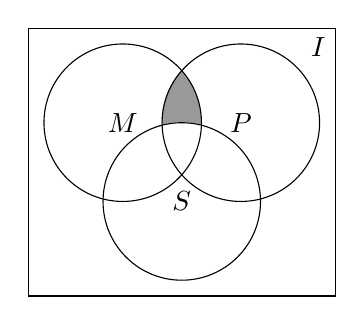
\begin{tikzpicture}
        \begin{scope}
            \clip (0,0) circle (1);
            \filldraw [gray!80] (1.5,0) circle (1);
        \end{scope}
        \filldraw [white] (0.75,-1) circle (1);
        \draw (0,0) circle (1) node {$M$};
        \draw (1.5,0) circle (1) node {$P$};
        \draw (0.75,-1) circle (1) node {$S$};
        \draw (-1.2,-2.2) rectangle (2.7,1.2) node [below left] {$I$};
    \end{tikzpicture}
\end{center}
\fourch{$(M\cap P)\cap S$}{$(M\cap P)\cup S$}{$(M\cap P)\cap \complement _IS$}{$(M\cap P)\cup \complement _IS$}


关联目标:

暂未关联目标



标签: 第一单元

答案: 暂无答案

解答或提示: 暂无解答与提示

使用记录:

暂无使用记录


出处: 二期课改练习册高一第一学期
\item { (007750)}若方程$x^2+px+4=0$的解集为$A$, 方程$x^2+x+q=0$的解集为$B$, 且$A\cap B=\{4\}$, 则集合$A\cup B$的所有子集是\blank{50}.


关联目标:

暂未关联目标



标签: 第一单元

答案: 暂无答案

解答或提示: 暂无解答与提示

使用记录:

暂无使用记录


出处: 二期课改练习册高一第一学期
\item { (007752)}已知集合$A=\{x|-2<x\le 1\}$, 集合$B=\{x|x\ge 1x<-2\}$, 求$A\cup B$, $A\cap B$.


关联目标:

暂未关联目标



标签: 第一单元

答案: 暂无答案

解答或提示: 暂无解答与提示

使用记录:

暂无使用记录


出处: 二期课改练习册高一第一学期
\item { (007753)}已知集合$A=\{x|-1<x<1$或$x\ge 3\}$, 集合$U=\{x|x\ge 2x<1\}$, 求$\complement _UA$.


关联目标:

暂未关联目标



标签: 第一单元

答案: 暂无答案

解答或提示: 暂无解答与提示

使用记录:

暂无使用记录


出处: 二期课改练习册高一第一学期
\item { (007755)}已知集合$A=\{x|x^2+px+q=0\}$, 集合$B=\{x|x^2-x+r=0\}$, 且$A\cap B=\{-1\}$, $A\cup B=\{-1,2\}$, 求$p$、$q$、$r$的值.


关联目标:

暂未关联目标



标签: 第一单元

答案: 暂无答案

解答或提示: 暂无解答与提示

使用记录:

暂无使用记录


出处: 二期课改练习册高一第一学期
\item { (007756)}已知全集$U=\mathbf{R}$, 集合$A=\{x|x\le a-1\}$, 集合$B=\{x|x>a+2\}$, 集合$C=\{x|x<0$或$x\ge 4\}$.若$\complement _U(A\cup B)\subseteq C$, 求实数$a$的取值范围.


关联目标:

暂未关联目标



标签: 第一单元

答案: 暂无答案

解答或提示: 暂无解答与提示

使用记录:

暂无使用记录


出处: 二期课改练习册高一第一学期
\item { (007757)}若集合$M=\{a|a=x+\sqrt 2y,\ x,y\in \mathbf{Q}\}$, 则下列结论正确的是\bracket{20}.
\fourch{$M\subseteq \mathbf{Q}$}{$M=\mathbf{Q}$}{$M\supsetneqq \mathbf{Q}$}{$M\subsetneqq \mathbf{Q}$}


关联目标:

暂未关联目标



标签: 第一单元

答案: 暂无答案

解答或提示: 暂无解答与提示

使用记录:

暂无使用记录


出处: 二期课改练习册高一第一学期
\item { (007760)}已知集合$P=\{x|-2\le x\le 5\}$, 集合$Q=\{x|k+1\le x\le 2k-1\}$, 且$Q\subseteq P$, 求实数$k$的取值范围.


关联目标:

暂未关联目标



标签: 第一单元

答案: 暂无答案

解答或提示: 暂无解答与提示

使用记录:

暂无使用记录


出处: 二期课改练习册高一第一学期
\item { (007761)}已知集合$A=\{x|(a-1)x^2+3x-2=0\}$, 是否存在这样的实数$a$, 使得集合$A$有且仅有两个子集? 若存在, 求出实数$a$的值及对应的两个子集;若不存在.请说明理由.


关联目标:

暂未关联目标



标签: 第一单元

答案: 暂无答案

解答或提示: 暂无解答与提示

使用记录:

暂无使用记录


出处: 二期课改练习册高一第一学期
\item { (007793)}已知集合$U=\mathbf{R}$, 且集合$A=\{x|x^2-16<0\}$, 集合$B=\{x|x^2-4x+3\ge 0\}$, 求:\\
(1) $A\cap B$;\\
(2) $A\cup B$;\\
(3) $\complement _U(A\cap B)$;\\
(4) $\complement _UA\cup \complement _UB$.


关联目标:

暂未关联目标



标签: 第一单元

答案: 暂无答案

解答或提示: 暂无解答与提示

使用记录:

暂无使用记录


出处: 二期课改练习册高一第一学期
\item { (007985)}若集合$A=\{x|0.1<\dfrac 1x<0.3,\ x\in \mathbf{N}\}$, 集合$B=\{x||x|\le 5,\ x\in \mathbf{Z}\}$, 则$A\cup B$中的元素个数是\bracket{20}.
\fourch{$11$}{$13$}{$15$}{$17$}


关联目标:

暂未关联目标



标签: 第一单元

答案: 暂无答案

解答或提示: 暂无解答与提示

使用记录:

暂无使用记录


出处: 二期课改练习册高一第一学期
\item { (007988)}已知集合$A=\{x|3x^2+x-2\ge 0,\  x\in \mathbf{R}\}$, 集合$B=\{x|\dfrac{4x-3}{x-3}>0,\ x\in \mathbf{R}\}$, 求$A\cap B$.


关联目标:

暂未关联目标



标签: 第一单元

答案: 暂无答案

解答或提示: 暂无解答与提示

使用记录:

暂无使用记录


出处: 二期课改练习册高一第一学期
\item { (007990)}已知集合$A=(-2,-1)\cup (0,+\infty)$, 集合$B=\{x|x^2+ax+b\le 0\}$, 且$A\cap B=(0,2]$, $A\cup B=(-2,+\infty)$, 求实数$a$、$b$的值.


关联目标:

暂未关联目标



标签: 第一单元

答案: 暂无答案

解答或提示: 暂无解答与提示

使用记录:

暂无使用记录


出处: 二期课改练习册高一第一学期
\item { (007995)}已知集合$A=\{x||x-a|<2\}$, 集合$B=\{x|\dfrac{2x-1}{x-2}<1\}$, 且$A\subseteq B$, 求实数$a$的取值范围.


关联目标:

暂未关联目标



标签: 第一单元

答案: 暂无答案

解答或提示: 暂无解答与提示

使用记录:

暂无使用记录


出处: 二期课改练习册高一第一学期
\item { (007996)}已知全集$U=\mathbf{R}$, 集合$A=\{x|x^2+px+12=0\}$, 集合$B=\{x|x-5x-q=0\}$, 满足$(\complement _UA)\cap B=\{2\}$.求实数$p$与$q$的值.


关联目标:

暂未关联目标



标签: 第一单元

答案: 暂无答案

解答或提示: 暂无解答与提示

使用记录:

暂无使用记录


出处: 二期课改练习册高一第一学期
\item { (009426)}判断下列各组对象能否组成集合. 若能组成集合, 指出是有限集还是无限集; 若不能组成集合, 请说明理由.\\
(1) 上海市现有各区的名称;\\
(2) 末位是$3$的自然数;\\
(3) 比较大的苹果.


关联目标:

暂未关联目标



标签: 第一单元

答案: 暂无答案

解答或提示: 暂无解答与提示

使用记录:

暂无使用记录


出处: 新教材必修第一册课堂练习
\item { (009428)}用列举法表示下列集合:\\
(1) 能整除$10$的所有正整数组成的集合;\\
(2) 绝对值小于$4$的所有整数组成的集合.


关联目标:

暂未关联目标



标签: 第一单元

答案: 暂无答案

解答或提示: 暂无解答与提示

使用记录:

暂无使用记录


出处: 新教材必修第一册课堂练习
\item { (009429)}用描述法表示下列集合:\\
(1) 全体偶数组成的集合;\\
(2) 平面直角坐标系中$x$轴上所有点组成的集合.


关联目标:

暂未关联目标



标签: 第一单元

答案: 暂无答案

解答或提示: 暂无解答与提示

使用记录:

暂无使用记录


出处: 新教材必修第一册课堂练习
\item { (009430)}用区间表示下列集合:\\
(1) $\{x|-1<x\le 5\}$;\\
(2) 不等式$-2x>6$的所有解组成的集合.


关联目标:

暂未关联目标



标签: 第一单元

答案: 暂无答案

解答或提示: 暂无解答与提示

使用记录:

暂无使用记录


出处: 新教材必修第一册课堂练习
\item { (009433)}写出所有满足$\{a\}\subset M\subset \{a, b, c, d\}$的集合$M$.


关联目标:

暂未关联目标



标签: 第一单元

答案: 暂无答案

解答或提示: 暂无解答与提示

使用记录:

暂无使用记录


出处: 新教材必修第一册课堂练习
\item { (009435)}已知全集为$\mathbf{R}$, 集合$A=\{x|-2<x\le 1\}$. 求$A$.


关联目标:

暂未关联目标



标签: 第一单元

答案: 暂无答案

解答或提示: 暂无解答与提示

使用记录:

暂无使用记录


出处: 新教材必修第一册课堂练习
\item { (009436)}已知集合$A=\{1, 2, 3, 4, 5\}$, $B=\{2, 4, 6, 8\}$, $C=\{3, 4, 5, 6\}$. 求:\\
(1) $(A\cap B)\cup C$, $(A\cup C)\cap (B\cup C)$;\\
(2) $(A\cup B)\cap C$, $(A\cap C)\cup (B\cap C)$.


关联目标:

暂未关联目标



标签: 第一单元

答案: 暂无答案

解答或提示: 暂无解答与提示

使用记录:

暂无使用记录


出处: 新教材必修第一册课堂练习
\item { (009438)}判断下列命题的真假, 并说明理由:\\
(1) 所有偶数都不是素数;\\
(2) $\{1\}$是$\{0, 1, 2\}$的真子集;\\
(3) $0$是$\{0, 1, 2\}$的真子集;\\
(4) 如果集合$A$是集合$B$的子集, 那么$B$不是$A$的子集.


关联目标:

暂未关联目标



标签: 第一单元

答案: 暂无答案

解答或提示: 暂无解答与提示

使用记录:

暂无使用记录


出处: 新教材必修第一册课堂练习
\item { (009996)}若集合$A=[-1,2)$, $B=\mathbf{Z}$, 则$A\cap B=$\bracket{20}.
\fourch{$\{-2,-1,0,1\}$}{$\{-1,0,1\}$}{$\{-1,0\}$}{$\{-1\}$}


关联目标:

暂未关联目标



标签: 第一单元

答案: 暂无答案

解答或提示: 暂无解答与提示

使用记录:

暂无使用记录


出处: 上海2022年秋季高考试题13
\item { (010017)}用列举法表示下列集合:\\
(1) $10$以内的所有素数组成的集合;\\
(2) $\{y|y=x-1,\  0\le x\le 3,\ x\in \mathbf{Z}\}$.


关联目标:

暂未关联目标



标签: 第一单元

答案: 暂无答案

解答或提示: 暂无解答与提示

使用记录:

暂无使用记录


出处: 新教材必修第一册习题
\item { (010018)}用描述法表示下列集合:\\
(1) 被$3$除余$1$的所有自然数组成的集合;\\
(2) 比$1$大又比$10$小的所有实数组成的集合;\\
(3) 平面直角坐标系中坐标轴上所有点组成的集合.


关联目标:

暂未关联目标



标签: 第一单元

答案: 暂无答案

解答或提示: 暂无解答与提示

使用记录:

暂无使用记录


出处: 新教材必修第一册习题
\item { (010019)}集合$\{(x, y)|xy>0, \ x,y\text{为实数}\}$是指\bracket{20}.
\twoch{第一象限内的所有点组成的集合}{第三象限内的所有点组成的集合}{第一象限和第三象限内的所有点组成的集合}{不在第二象限也不在第四象限内的所有点组成的集合}


关联目标:

暂未关联目标



标签: 第一单元

答案: 暂无答案

解答或提示: 暂无解答与提示

使用记录:

暂无使用记录


出处: 新教材必修第一册习题
\item { (010020)}用符号``$\subset$''``$=$''或``$\supset$''连接集合$A$与$B$:\\
(1) $A=\{x|x^2-2x+1=0\}$, $B=\{x|x^2-1=0\}$;\\
(2) $A=\{1, 2, 4, 8\}$, $B=\{x|x$是$8$的正约数$\}$.


关联目标:

暂未关联目标



标签: 第一单元

答案: 暂无答案

解答或提示: 暂无解答与提示

使用记录:

暂无使用记录


出处: 新教材必修第一册习题
\item { (010021)}已知集合$A=\{1\}$, $B=\{x|x^2-3x+a=0\}$. 是否存在实数$a$, 使得$A\subset B$?  若存在, 求$a$的值; 若不存在, 说明理由.


关联目标:

暂未关联目标



标签: 第一单元

答案: 暂无答案

解答或提示: 暂无解答与提示

使用记录:

暂无使用记录


出处: 新教材必修第一册习题
\item { (010022)}已知集合$A=\{x, y\}$, $B=\{2x, 2x^2\}$, 且$A=B$. 求集合$A$.


关联目标:

暂未关联目标



标签: 第一单元

答案: 暂无答案

解答或提示: 暂无解答与提示

使用记录:

暂无使用记录


出处: 新教材必修第一册习题
\item { (010023)}已知集合$A=\{x|x\le 7\}$, $B=\{x|x<2\}$, $C=\{x|x>5\}$. 求: $A\cap B$, $A\cap C$, $A\cap (B\cap C)$.


关联目标:

暂未关联目标



标签: 第一单元

答案: 暂无答案

解答或提示: 暂无解答与提示

使用记录:

暂无使用记录


出处: 新教材必修第一册习题
\item { (010024)}已知集合$A=\{(x, y)|y=-x+1\}$, $B=\{(x, y)|y=x^2-1\}$. 求$A\cap B$.


关联目标:

暂未关联目标



标签: 第一单元

答案: 暂无答案

解答或提示: 暂无解答与提示

使用记录:

暂无使用记录


出处: 新教材必修第一册习题
\item { (010025)}已知全集$U=\mathbf{R}$, 集合$A=\{x|4-x>2x+1\}$. 求$\overline A$.


关联目标:

暂未关联目标



标签: 第一单元

答案: 暂无答案

解答或提示: 暂无解答与提示

使用记录:

暂无使用记录


出处: 新教材必修第一册习题
\item { (010026)}已知集合$A=\{2, (a+1)^2, a^2+3a+3\}$, 且$1\in A$. 求实数$a$的值.


关联目标:

暂未关联目标



标签: 第一单元

答案: 暂无答案

解答或提示: 暂无解答与提示

使用记录:

暂无使用记录


出处: 新教材必修第一册习题
\item { (010027)}已知集合$A=\{x|x=2n+1,\ n\in \mathbf{Z}\}$, $B=\{x|x=4n-1,\ n\in \mathbf{Z}\}$. 判断集合$A$与$B$的包含关系, 并证明你的结论.


关联目标:

暂未关联目标



标签: 第一单元

答案: 暂无答案

解答或提示: 暂无解答与提示

使用记录:

暂无使用记录


出处: 新教材必修第一册习题
\item { (010028)}设$a$是实数, 集合$M=\{x|x^2+x-6=0\}$, $N=\{y|ay+2=0\}$. 是否存在$a$, 使得$N\subset M$? 若存在, 求这些$a$的值; 若不存在, 说明理由.


关联目标:

暂未关联目标



标签: 第一单元

答案: 暂无答案

解答或提示: 暂无解答与提示

使用记录:

暂无使用记录


出处: 新教材必修第一册习题
\item { (010029)}已知集合$A=\{1, 4, x\}$, $B=\{1, x^2\}$, 且$A\cup B=A$. 求$x$的值及集合$A$、$B$.


关联目标:

暂未关联目标



标签: 第一单元

答案: 暂无答案

解答或提示: 暂无解答与提示

使用记录:

暂无使用记录


出处: 新教材必修第一册习题
\item { (010033)}下列各组中, $\alpha$是$\beta$的什么条件?\\
(1) $\alpha$: 四边形$ABCD$的四条边等长, $\beta$: 四边形$ABCD$是正方形;\\
(2) $\alpha$: $\triangle ABC$与$\triangle DEF$全等, $\beta$: $\triangle ABC$与$\triangle DEF$的周长相等;\\
(3) $\alpha$: $x$是$2$的倍数, $\beta$: $x$是$6$的倍数;\\
(4) $\alpha$: 集合$A\subseteq B$, $B\subseteq C$, $C\subseteq A$, $\beta$: 集合$A=B=C$;\\
(5) $\alpha$: $A\cap B=A\cap C$, $\beta$: $B=C$.


关联目标:

暂未关联目标



标签: 第一单元

答案: 暂无答案

解答或提示: 暂无解答与提示

使用记录:

暂无使用记录


出处: 新教材必修第一册习题
\item { (010069)}设全集为$\mathbf{R}$, 集合$A=\{x|x^2-2x-3\ge 0\}$
, $B=\{x|x^2+x-2<0\}$. 求:\\
(1) $A\cup B$;\\
(2) $A\cap B$;\\
(3) $\overline{A\cap B}$;\\
(4) $\overline A\cup \overline B$.


关联目标:

暂未关联目标



标签: 第一单元

答案: 暂无答案

解答或提示: 暂无解答与提示

使用记录:

暂无使用记录


出处: 新教材必修第一册习题
\item { (020001)}判断下列各组对象能否组成集合, 若能组成集合, 指出是有限集还是无限集.\\
(1) 上海市控江中学$2022$年入学的全体高一年级新生;\\
(2) 中国现有各省的名称;\\
(3) 太阳、$2$、上海市;\\
(4) 大于$10$且小于$15$的有理数;\\
(5) 末位是$3$的自然数;\\
(6) 影响力比较大的中国数学家;\\
(7) 方程$x^2+x+3=0$的所有实数解;\\ 
(8) 函数$y=\dfrac 1x$图像上所有的点;\\ 
(9) 在平面直角坐标系中, 到定点$(0, 0)$的距离等于$1$的所有点;\\
(10) 不等式$3x-10<0$的所有正整数解;\\
(11) 所有的平面四边形.


关联目标:

暂未关联目标



标签: 第一单元

答案: 暂无答案

解答或提示: 暂无解答与提示

使用记录:

暂无使用记录


出处: 2025届高一校本作业必修第一章
\item { (020003)}对于一个确定的实数$x$, 由$x$, $-x$, $|x|$, $-\sqrt{x^2}$中的一个值或几个值组成的所有集合中, 元素的个数最多有多少个?


关联目标:

暂未关联目标



标签: 第一单元

答案: 暂无答案

解答或提示: 暂无解答与提示

使用记录:

暂无使用记录


出处: 2025届高一校本作业必修第一章
\item { (020004)}已知关于$x$的方程$\sqrt {x^2+4x+a}=x+2$, 若以该方程的所有解为元素组成的集合是无限集, 求实数$a$满足的条件.


关联目标:

暂未关联目标



标签: 第一单元

答案: 暂无答案

解答或提示: 暂无解答与提示

使用记录:

暂无使用记录


出处: 2025届高一校本作业必修第一章
\item { (020005)}用列举法表示下列集合:\\
(1) $12$以内的素数组成的集合;\\
(2) 绝对值小于$3$的所有整数的集合;\\
(3) $\{x|\dfrac 6{3-x}\in\mathbf{N}, \ x\in\mathbf{Z}\}$;\\
(4) $\{y|y=x^2-1 , \ |x| \le 2, \ x\in\mathbf{Z}\}$;\\
(5) $\{( x,y)|y=x^2-1,\ |x|\le 2, \ x\in\mathbf{Z}\}$;\\
(6) $\{( x,y)|x +y=5, \ x\in\mathbf{N}, \ y\in\mathbf{N}\}$.


关联目标:

暂未关联目标



标签: 第一单元

答案: 暂无答案

解答或提示: 暂无解答与提示

使用记录:

暂无使用记录


出处: 2025届高一校本作业必修第一章
\item { (020006)}用描述法表示下列集合:\\
(1) 所有奇数组成的集合;\\
(2) 被$3$除余数等于$2$的正整数的集合;\\
(3) 不小于$10$的实数组成的集合;\\
(4) 绝对值大于$4$的所有整数组成的集合;\\
(5) 平面直角坐标系内$y$轴上的点的坐标组成的集合;\\
(6) 在直线$y=2x+1$上所有的点的坐标组成的集合.


关联目标:

暂未关联目标



标签: 第一单元

答案: 暂无答案

解答或提示: 暂无解答与提示

使用记录:

暂无使用记录


出处: 2025届高一校本作业必修第一章
\item { (020007)}用区间表示下列集合:\\
(1) $\{x|-2<x<7\}$;\\
(2) $\{x|-2\le\ x\le7\}$;\\
(3) $\{x|-2\le\ x<7\}$;\\
(4) 不等式$2x<5$的解集;\\
(5) 不等式$-x<5$的解集; \\
(6) 非负实数集.


关联目标:

暂未关联目标



标签: 第一单元

答案: 暂无答案

解答或提示: 暂无解答与提示

使用记录:

暂无使用记录


出处: 2025届高一校本作业必修第一章
\item { (020008)}用适当的方法表示下列集合:\\
(1) 能被$10$整除的所有正整数组成的集合;\\
(2) 能整除$10$的所有正整数组成的集合;\\
(3) 方程$x^2+2=0$的实数解组成的集合;\\
(4) 方程组$\begin{cases}2x+y=0, \\ x-y+3=0\end{cases}$的所有解组成的集合;\\
(5) 两直线$y=2x+1$和$y=x-2$的交点组成的集合.


关联目标:

暂未关联目标



标签: 第一单元

答案: 暂无答案

解答或提示: 暂无解答与提示

使用记录:

暂无使用记录


出处: 2025届高一校本作业必修第一章
\item { (020010)}集合$\{(x, y)|xy\ge 0,\  x\in\mathbf{R},\  y\in\mathbf{R}\}$是指\bracket{20}.
\twoch{第一象限内的所有点}{第三象限内的所有点}{第一象限和第三象限内的所有点}{不在第二象限、第四象限内的所有点}


关联目标:

暂未关联目标



标签: 第一单元

答案: 暂无答案

解答或提示: 暂无解答与提示

使用记录:

暂无使用记录


出处: 2025届高一校本作业必修第一章
\item { (020011)}若集合$M=\{0,2,3,7\}$, $P=\{x|x=ab,\ a,b\in M, \ a\ne b\}$. 用列举法写出集合$P$.


关联目标:

暂未关联目标



标签: 第一单元

答案: 暂无答案

解答或提示: 暂无解答与提示

使用记录:

暂无使用记录


出处: 2025届高一校本作业必修第一章
\item { (020012)}已知集合$A={2, a^2, a}$, 且$1\in A$, 求实数$a$的值.


关联目标:

暂未关联目标



标签: 第一单元

答案: 暂无答案

解答或提示: 暂无解答与提示

使用记录:

暂无使用记录


出处: 2025届高一校本作业必修第一章
\item { (020013)}设集合$M=\{a|a=x^2-y^2, \ x,y\in\mathbf{Z}\}$, 下列数中不属于$M$的为\bracket{20}.
\fourch{$3$}{$6$}{$9$}{$12$}


关联目标:

暂未关联目标



标签: 第一单元

答案: 暂无答案

解答或提示: 暂无解答与提示

使用记录:

暂无使用记录


出处: 2025届高一校本作业必修第一章
\item { (020014)}已知集合$A=\{x|x=a+\sqrt 2b,\ a,b\in \mathbf{Z}\}$, 若$x_1,x_2\in A$, 证明: $x_1x_2\in A$.


关联目标:

暂未关联目标



标签: 第一单元

答案: 暂无答案

解答或提示: 暂无解答与提示

使用记录:

暂无使用记录


出处: 2025届高一校本作业必修第一章
\item { (020015)}已知集合$A=\{x|(k+1)x^2+x-k=0\}$中只有一个元素, 求实数$k$的值.


关联目标:

暂未关联目标



标签: 第一单元

答案: 暂无答案

解答或提示: 暂无解答与提示

使用记录:

暂无使用记录


出处: 2025届高一校本作业必修第一章
\item { (020017)}集合$\{1,2,3\}$的子集共有\blank{50}个.


关联目标:

暂未关联目标



标签: 第一单元

答案: 暂无答案

解答或提示: 暂无解答与提示

使用记录:

暂无使用记录


出处: 2025届高一校本作业必修第一章
\item { (020018)}已知集合$A=\{1,2\}$, 集合$B=\{1,2,3,4,5\}$. 若集合$M$满足$A\subset M$且$M\subseteq B$, 则这样的集合$M$有\blank{50}个.


关联目标:

暂未关联目标



标签: 第一单元

答案: 暂无答案

解答或提示: 暂无解答与提示

使用记录:

暂无使用记录


出处: 2025届高一校本作业必修第一章
\item { (020019)}满足$\{a, b\}\subset M \subset\{a, b, c, d, e\}$的集合$M$有\blank{50}个.


关联目标:

暂未关联目标



标签: 第一单元

答案: 暂无答案

解答或提示: 暂无解答与提示

使用记录:

暂无使用记录


出处: 2025届高一校本作业必修第一章
\item { (020021)}下列各选项中, $M$与$P$表示同一个集合的有\blank{50}.\\
\textcircled{1} $M=\{(1, -3)\}$, $P=\{(-3, 1)\}$; \textcircled{2} $M=\{1, -3\}$, $P=\{-3, 1\}$; \textcircled{3} $M=\varnothing$, $P=\{\varnothing\}$; \textcircled{4} $M=\{y|y=x^2+1, \  x\in\mathbf{R}\}$, $P=\{(x, y)|y=x^2+1, \ x\in\mathbf{R}\}$; \textcircled{5} $M=\{y|y=x^2+1, \  x\in\mathbf{R}\}$, $P=\{t|t=y^2+1, \ y\in\mathbf{R}\}$; \textcircled{6} $M=\{y|y=x^2+1, \  x\in\mathbf{R}\}$, $P=\{x|y=\sqrt{x-1},\  x\in\mathbf{R}\}$.


关联目标:

暂未关联目标



标签: 第一单元

答案: 暂无答案

解答或提示: 暂无解答与提示

使用记录:

暂无使用记录


出处: 2025届高一校本作业必修第一章
\item { (020023)}设常数$x,y\in \mathbf{R}$, 已知集合$A=\{x, y\}$, $B=\{2x, x^2\}$, 且$A=B$, 求集合$A$.


关联目标:

暂未关联目标



标签: 第一单元

答案: 暂无答案

解答或提示: 暂无解答与提示

使用记录:

暂无使用记录


出处: 2025届高一校本作业必修第一章
\item { (020024)}证明:集合$A=\{1,2,3\}$是集合$B=\{0,1,2,3,4,5,6\}$的子集.


关联目标:

暂未关联目标



标签: 第一单元

答案: 暂无答案

解答或提示: 暂无解答与提示

使用记录:

暂无使用记录


出处: 2025届高一校本作业必修第一章
\item { (020025)}判断集合$A=\{n|n=2k-1,\ k\in \mathbf{Z}\}$, $B=\{n|n=2m+1,m\in \mathbf{Z}\}$的关系, 并说明理由.


关联目标:

暂未关联目标



标签: 第一单元

答案: 暂无答案

解答或提示: 暂无解答与提示

使用记录:

暂无使用记录


出处: 2025届高一校本作业必修第一章
\item { (020026)}证明集合$A=\{n|n=2k-1,\ k\in \mathbf{N}\}$不是集合$B=\{n|n=2m+1, \ m\in \mathbf{N}\}$的子集, 且集合$A$真包含集合$B$.


关联目标:

暂未关联目标



标签: 第一单元

答案: 暂无答案

解答或提示: 暂无解答与提示

使用记录:

暂无使用记录


出处: 2025届高一校本作业必修第一章
\item { (020027)}已知集$B=\{0, 2, 4\}$, $C=\{0, 2, 6\}$, 若集合$A$满足$A\subseteq B$, $A\subseteq C$, 写出所有满足条件的集合$A$.


关联目标:

暂未关联目标



标签: 第一单元

答案: 暂无答案

解答或提示: 暂无解答与提示

使用记录:

暂无使用记录


出处: 2025届高一校本作业必修第一章
\item { (020028)}已知集合$A=\{1\}$, $B=\{x|x\subseteq A\}$, 用列举法表示集合$B$. 并指出$A$与$B$的关系.


关联目标:

暂未关联目标



标签: 第一单元

答案: 暂无答案

解答或提示: 暂无解答与提示

使用记录:

暂无使用记录


出处: 2025届高一校本作业必修第一章
\item { (020029)}若集合$A=\{2,a,a+3\}$, $B=\{2,3,5,8\}$, 且$B\supset A$, 则$a$的值为\blank{50}.


关联目标:

暂未关联目标



标签: 第一单元

答案: 暂无答案

解答或提示: 暂无解答与提示

使用记录:

暂无使用记录


出处: 2025届高一校本作业必修第一章
\item { (020030)}设常数$a\in \mathbf{R}$. 若集合$A=(-\infty ,5)$与$B=(-\infty ,a]$满足$A\subseteq B$, 则$a$的取值范围是\blank{50}.\\
证明: $1^\circ$ 当$a$\blank{50}时, 任取$x\in A$, 则\blank{50}, 所以$x\in B$, 即$A\subseteq B$.\\ 
$2^\circ$ 当$a$\blank{50}时, 取$x_1=$\blank{50}, 则\blank{50}, 所以$x_1\in A$且$x_1\not \in B$.\\
由$1^\circ$、$2^\circ$可得结论.


关联目标:

暂未关联目标



标签: 第一单元

答案: 暂无答案

解答或提示: 暂无解答与提示

使用记录:

暂无使用记录


出处: 2025届高一校本作业必修第一章
\item { (020032)}已知集合$A=\{1\}$, 集合$B=\{x|x^2-2x+a=0\}$, 且$A\subset B$, 求实数$a$的取值范围.


关联目标:

暂未关联目标



标签: 第一单元

答案: 暂无答案

解答或提示: 暂无解答与提示

使用记录:

暂无使用记录


出处: 2025届高一校本作业必修第一章
\item { (020033)}已知集合$S=\{1, 2\}$, 集合$T=\{x|ax^2-3x+2=0\}$, 且$S=T$, 求实数$a$的取值范围.


关联目标:

暂未关联目标



标签: 第一单元

答案: 暂无答案

解答或提示: 暂无解答与提示

使用记录:

暂无使用记录


出处: 2025届高一校本作业必修第一章
\item { (020034)}已知集合$S=\{1, 2\}$, 集合$T=\{x|ax^2-3x+2=0\}$, 且$S\supseteq T$, 求实数$a$的取值范围.


关联目标:

暂未关联目标



标签: 第一单元

答案: 暂无答案

解答或提示: 暂无解答与提示

使用记录:

暂无使用记录


出处: 2025届高一校本作业必修第一章
\item { (020035)}证明:集合$A=\{x|x=6n-1, \ n\in\mathbf{Z}\}$是$B=\{x|x=3n+2, \ n\in\mathbf{Z}\}$的真子集.


关联目标:

暂未关联目标



标签: 第一单元

答案: 暂无答案

解答或提示: 暂无解答与提示

使用记录:

暂无使用记录


出处: 2025届高一校本作业必修第一章
\item { (020036)}设常数$a\in \mathbf{R}$, 已知集合$\{A=x|x^2-1=0\}$, 集合$\{B=x|(x-1)(x-a)=0\}$.
(1) 若$B\subset A$, 求$a$值的集合;\\
(2) 若$B$不是$A$的子集, 求$a$值的集合.


关联目标:

暂未关联目标



标签: 第一单元

答案: 暂无答案

解答或提示: 暂无解答与提示

使用记录:

暂无使用记录


出处: 2025届高一校本作业必修第一章
\item { (020037)}已知集合$A=\{x|0<x<a\}$, $B=\{x|1<x<2\}$, 若$B\subseteq A$, 则实数$a$的取值范围为\blank{50}.


关联目标:

暂未关联目标



标签: 第一单元

答案: 暂无答案

解答或提示: 暂无解答与提示

使用记录:

暂无使用记录


出处: 2025届高一校本作业必修第一章
\item { (020038)}已知集合$A=[-2,5]$, $B=[m+1,2m-1]$, 满足$B\subseteq A$, 则实数$m$的取值范围为\blank{50}.


关联目标:

暂未关联目标



标签: 第一单元

答案: 暂无答案

解答或提示: 暂无解答与提示

使用记录:

暂无使用记录


出处: 2025届高一校本作业必修第一章
\item { (020039)}已知非空集合$P$满足: \textcircled{1} $P\subseteq \{1,2,3,4,5\}$; \textcircled{2} 若$a\in P$, 则$6-a\in P$, 符合上述要求的集合$P$的个数是\blank{50}.


关联目标:

暂未关联目标



标签: 第一单元

答案: 暂无答案

解答或提示: 暂无解答与提示

使用记录:

暂无使用记录


出处: 2025届高一校本作业必修第一章
\item { (020040)}已知集合$A=\{1, 1+d, 1+3d\}$, 集合$B=\{1, q, q^2\}$, 其中$d$、$q\in \mathbf{R}$, 且$d\ne 0$. 若$A=B$, 求$q$的值.


关联目标:

暂未关联目标



标签: 第一单元

答案: 暂无答案

解答或提示: 暂无解答与提示

使用记录:

暂无使用记录


出处: 2025届高一校本作业必修第一章
\item { (020041)}已知$A=\{x|x=a+\sqrt 2b,\ a,b\in \mathbf{N}\}$, 若集合$B=\{x|x=\sqrt 2x_1,\  x_1 \in A\}$, 证明$B\subset A$.


关联目标:

暂未关联目标



标签: 第一单元

答案: 暂无答案

解答或提示: 暂无解答与提示

使用记录:

暂无使用记录


出处: 2025届高一校本作业必修第一章
\item { (020043)}已知任一集合$A$, 则\\
(1) $A\cap A=$\blank{50};\\
(2) $A\cap\varnothing=$\blank{50};\\
(3) $A\cup A=$\blank{50};\\
(4) $A\cup\varnothing=$\blank{50}.


关联目标:

暂未关联目标



标签: 第一单元

答案: 暂无答案

解答或提示: 暂无解答与提示

使用记录:

暂无使用记录


出处: 2025届高一校本作业必修第一章
\item { (020050)}已知集合$A=\{x| x\le 1\}$, 集合 $B=\{x| x\ge a\}$, 且$A\cup B=\mathbf{R}$, 则$a$的取值范围为\blank{50}.


关联目标:

暂未关联目标



标签: 第一单元

答案: 暂无答案

解答或提示: 暂无解答与提示

使用记录:

暂无使用记录


出处: 2025届高一校本作业必修第一章
\item { (020051)}设常数$a\in \mathbf{R}$. 已知集合$A=\{x|x^2-3x+2=0, \ x\in\mathbf{R}\}$, 集合$B=\{x|2x^2-x+2a=0,\  x\in\mathbf{R}\}$.\\ (1) 若$A\cup B=B$, 求$a$的值的集合;\\
(2) 若$A\cap B=B$, 求$a$的值的集合.


关联目标:

暂未关联目标



标签: 第一单元

答案: 暂无答案

解答或提示: 暂无解答与提示

使用记录:

暂无使用记录


出处: 2025届高一校本作业必修第一章
\item { (020052)}已知集合$A=(-\infty, -1)\cup(6, +\infty)$, 集合$B=(5-a, 5+a)$. 若$11\in B$, 则$A\cup B=$\blank{50}.


关联目标:

暂未关联目标



标签: 第一单元

答案: 暂无答案

解答或提示: 暂无解答与提示

使用记录:

暂无使用记录


出处: 2025届高一校本作业必修第一章
\item { (020053)}已知集合$P=\{ x|-2\le x\le 5\}$, $Q=\{x|x>k+1$且$x<2k-1\}$, 若$P\cap Q=\varnothing$, 求实数$k$的取值范围.


关联目标:

暂未关联目标



标签: 第一单元

答案: 暂无答案

解答或提示: 暂无解答与提示

使用记录:

暂无使用记录


出处: 2025届高一校本作业必修第一章
\item { (020054)}已知集合$A={(x, y)|x+y=0}$, 集合$B=\{(x,y)|y=x-2\}$, 集合$C=\{(x,y)|y=x+b\}$. 若$(A\cup C)\cap(B\cup C)=C$, 求实数$b$.


关联目标:

暂未关联目标



标签: 第一单元

答案: 暂无答案

解答或提示: 暂无解答与提示

使用记录:

暂无使用记录


出处: 2025届高一校本作业必修第一章
\item { (020055)}设常数$m\in \mathbf{R}$. 若集合$A=\{1,2,3\}$, 集合$B=\{m^2,3\}$, 且$A\cup B=\{1,2,3,m\}$, 则$m$的值是\blank{50}.


关联目标:

暂未关联目标



标签: 第一单元

答案: 暂无答案

解答或提示: 暂无解答与提示

使用记录:

暂无使用记录


出处: 2025届高一校本作业必修第一章
\item { (020056)}设常数$a\in \mathbf{R}$. 已知集合$A=\{x| x\le 1\}$, 集合$B=\{x| x>a\}$, 且$A\cap B=\varnothing$, 则$a$的取值范围为\blank{50}.


关联目标:

暂未关联目标



标签: 第一单元

答案: 暂无答案

解答或提示: 暂无解答与提示

使用记录:

暂无使用记录


出处: 2025届高一校本作业必修第一章
\item { (020060)}已知集合$U=\{x|x\ge 2\}$, 集合$A=\{y|3\le y<4\}$, 集合$B=\{z|2\le z<5\}$, 则$\overline A\cap B=$\blank{50}; $\overline B\cup A=$\blank{50}.


关联目标:

暂未关联目标



标签: 第一单元

答案: 暂无答案

解答或提示: 暂无解答与提示

使用记录:

暂无使用记录


出处: 2025届高一校本作业必修第一章
\item { (020063)}设常数$a\in \mathbf{R}$, 已知全集$U=\mathbf{R}$, 集合$A=\{x|-2<x<2\}$, 集合$B=\{x|x>a\}$. 若$A\cap\overline B=A$, 则$a$的取值范围为\blank{50}.


关联目标:

暂未关联目标



标签: 第一单元

答案: 暂无答案

解答或提示: 暂无解答与提示

使用记录:

暂无使用记录


出处: 2025届高一校本作业必修第一章
\item { (020064)}设常数$a\in \mathbf{R}$, 全集$U=\mathbf{R}$. 集合$A=\{x| x<2 \}$, $B=\{x| x>a \}$. 若$\overline A\subseteq B$, 则$a$的取值范围为\blank{50}.


关联目标:

暂未关联目标



标签: 第一单元

答案: 暂无答案

解答或提示: 暂无解答与提示

使用记录:

暂无使用记录


出处: 2025届高一校本作业必修第一章
\item { (020065)}用集合$A$、$B$的运算式表示图中的阴影部分:\\
(1) 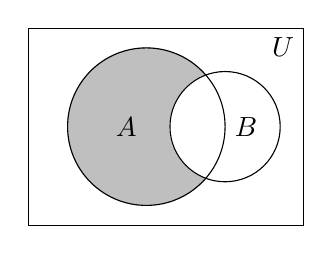
\begin{tikzpicture}
\draw (0,0) rectangle (3.5,2.5) node [below left] {$U$};
\filldraw [gray!50] (1.5,1.25) circle (1);
\filldraw [white] (2.5,1.25) circle (0.7);
\draw (1.5,1.25) circle (1) node [left] {$A$};
\draw (2.5,1.25) circle (0.7) node [right] {$B$};
\end{tikzpicture}\\
(2) 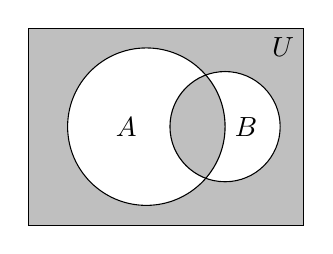
\begin{tikzpicture}
\filldraw [gray!50] (0,0) rectangle (3.5,2.5);
\draw (0,0) rectangle (3.5,2.5) node [below left] {$U$};
\filldraw [white] (1.5,1.25) circle (1);
\filldraw [white] (2.5,1.25) circle (0.7);
\begin{scope}
    \clip (1.5,1.25) circle (1);
    \clip (2.5,1.25) circle (0.7);
    \filldraw [gray!50] (0,0) rectangle (3.5,2.5);
\end{scope}
\draw (1.5,1.25) circle (1) node [left] {$A$};
\draw (2.5,1.25) circle (0.7) node [right] {$B$};
\end{tikzpicture}\\
(3) 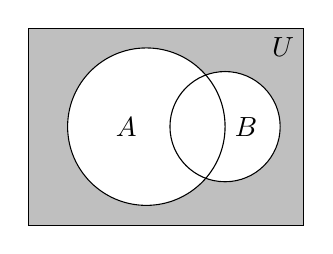
\begin{tikzpicture}
\filldraw [gray!50] (0,0) rectangle (3.5,2.5);
\draw (0,0) rectangle (3.5,2.5) node [below left] {$U$};
\filldraw [white] (1.5,1.25) circle (1);
\filldraw [white] (2.5,1.25) circle (0.7);
\draw (1.5,1.25) circle (1) node [left] {$A$};
\draw (2.5,1.25) circle (0.7) node [right] {$B$};
\end{tikzpicture}


关联目标:

暂未关联目标



标签: 第一单元

答案: 暂无答案

解答或提示: 暂无解答与提示

使用记录:

暂无使用记录


出处: 2025届高一校本作业必修第一章
\item { (020067)}已知全集$U=A\cup B=\{x|0\le x\le 10, \ x\in \mathbf{N}\}$, $A\cap\overline B=\{1, 3, 5, 7\}$. 则集合$B=$\blank{50}.


关联目标:

暂未关联目标



标签: 第一单元

答案: 暂无答案

解答或提示: 暂无解答与提示

使用记录:

暂无使用记录


出处: 2025届高一校本作业必修第一章
\item { (020068)}若全集$U=\{(x,y)|x\in\mathbf{R},\ y\in\mathbf{R}\}$, 集合$A=\{(x,y)|\dfrac yx=1\}$, 集合$B=\{(x,y)|y\neq x\}$, 则$\overline{A\cup B}= $\blank{50}.


关联目标:

暂未关联目标



标签: 第一单元

答案: 暂无答案

解答或提示: 暂无解答与提示

使用记录:

暂无使用记录


出处: 2025届高一校本作业必修第一章
\item { (020069)}如图, 已知集合$U$为全集, 分别用集合$A$、$B$、$C$的运算式表示下列图中的阴影部分.
\begin{center}
    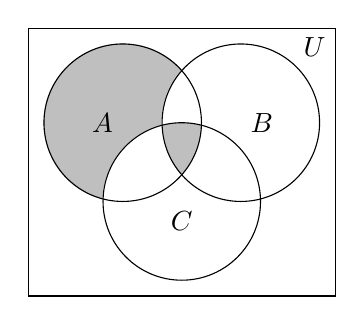
\begin{tikzpicture}
        \filldraw [gray!50] (0,0) circle (1);
        \filldraw [white] (1.5,0) circle (1);
        \filldraw [white] (0.75,-1) circle (1);
        \begin{scope}
            \clip (0,0) circle (1);
            \clip (1.5,0) circle (1);
            \clip (0.75,-1) circle (1);
            \filldraw [gray!50] (1.5,0) circle (1);
        \end{scope}
        \draw (0,0) circle (1) node [left] {$A$};
        \draw (1.5,0) circle (1) node [right] {$B$};
        \draw (0.75,-1) circle (1) node [below] {$C$};
        \draw (-1.2,-2.2) rectangle (2.7,1.2) node [below left] {$U$};
    \end{tikzpicture}
    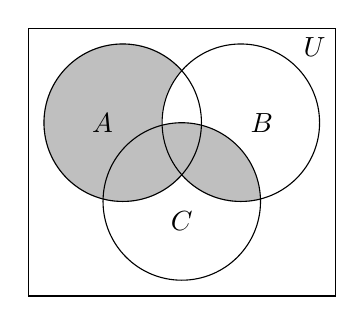
\begin{tikzpicture}
        \filldraw [gray!50] (0,0) circle (1);
        \filldraw [white] (1.5,0) circle (1);
        \begin{scope}
            \clip (0.75,-1) circle (1);
            \filldraw [gray!50] (1.5,0) circle (1);
        \end{scope}
        \draw (0,0) circle (1) node [left] {$A$};
        \draw (1.5,0) circle (1) node [right] {$B$};
        \draw (0.75,-1) circle (1) node [below] {$C$};
        \draw (-1.2,-2.2) rectangle (2.7,1.2) node [below left] {$U$};
    \end{tikzpicture}
\end{center}


关联目标:

暂未关联目标



标签: 第一单元

答案: 暂无答案

解答或提示: 暂无解答与提示

使用记录:

暂无使用记录


出处: 2025届高一校本作业必修第一章
\item { (020071)}判断下列命题的真假, 并在相应的括号内填入``真''或``假''.\\
(1) $2\sqrt 3>3\sqrt 2$或$1\le 1$;\blank{50};\\
(2) $2\sqrt 3>3\sqrt 2$且$1\le1$;\blank{50};\\
(3) 如果$a$、$b$都是奇数, 那么$ab$也是奇数;\blank{50};\\
(4) $\{1\}$是$\{0, 1, 2\}$的真子集;\blank{50};\\
(5) $1$是$\{0, 1, 2\}$的真子集;\blank{50};\\
(6) 若$x<-2$或$x>2$, 则$x^2>1$;\blank{50};\\
(7) 如果$|a|<2$, 那么$a<2$;\blank{50};\\
(8) 对任意实数$a,b$, 方程$(a+1)x+b=0$的解为$x=-\dfrac b{a+1}$;\blank{50};\\
(9) 若命题$\alpha$、$\beta$、$\gamma$满足$\alpha\Rightarrow \beta$, $\beta\Rightarrow \gamma$, $\gamma\Rightarrow \alpha$, 则$\alpha\Leftrightarrow \gamma$;\blank{50};\\
(10) 若关于$x$的方程$ax^2+bx+c=0$($a\ne 0$)的两实数根之积是正数, 则$ac>0$;\blank{50};\\
(11) 若某个整数不是偶数, 则这个数不能被$4$整除;\blank{50};\\
(12) 合数一定是偶数;\blank{50};\\
(13) 所有的偶数都是素数或合数;\blank{50};\\
(14) 所有的偶数都是素数或所有的偶数都是合数;\blank{50};\\
(15) 如果$A\subset B$, $B\supset C$, 那么$A=C$;\blank{50};\\
(16) 空集是任何集合的真子集;\blank{50};\\
(17) 若$x\in \mathbf{R}$, 则方程$x^2-x+1=0$不成立;\blank{50};\\
(18) 若$A\cap B\ne \varnothing$, $B\subset C$, 则$A\cap C\ne \varnothing$;\blank{50};\\
(19) 存在一个三角形, 它的任意两边的平方和小于第三边的平方;\blank{50};\\
(20) 对于任意一个三角形, 存在一组两边的平方和不等于第三边的平方;\blank{50}.


关联目标:

暂未关联目标



标签: 第一单元

答案: 暂无答案

解答或提示: 暂无解答与提示

使用记录:

暂无使用记录


出处: 2025届高一校本作业必修第一章
\item { (020073)}已知命题``非空集合$M$的元素都是集合$P$的元素$''$是假命题, 给出下列命题: \textcircled{1} $M$中的元素都不是$P$的元素; \textcircled{2} $M$中有不属于$P$的元素; \textcircled{3} $M$中有$P$的元素; \textcircled{4} $M$中的元素不都是$P$的元素. 其中真命题有\blank{50}.


关联目标:

暂未关联目标



标签: 第一单元

答案: 暂无答案

解答或提示: 暂无解答与提示

使用记录:

暂无使用记录


出处: 2025届高一校本作业必修第一章
\item { (020084)}有限集合$S$中元素的个数记作$\mathrm{card}(S)$, 设$A,B$都是有限集合, 给出下列命题:\\
\textcircled{1} $A\cap B=\varnothing$的一个充要条件是$\mathrm{card}(A\cup B)=\mathrm{card}(A)+\mathrm{card}(B)$;\\
\textcircled{2} $A\subseteq B$的一个必要不充分条件是$\mathrm{card}(A)\le \mathrm{card}(B)$; \\
\textcircled{3} $A$不是$B$的子集的一个充分不必要条件是$\mathrm{card}(A)>\mathrm{card}(B)$;\\ 
\textcircled{4} $A=B$的一个充要条件是$\mathrm{card}(A)=\mathrm{card}(B)$.\\ 
其中真命题的个数是\bracket{20}.
\fourch{$0$}{$1$}{$2$}{$3$}


关联目标:

暂未关联目标



标签: 第一单元

答案: 暂无答案

解答或提示: 暂无解答与提示

使用记录:

暂无使用记录


出处: 2025届高一校本作业必修第一章
\end{enumerate}



\end{document}